%!TEX TS-program = xelatex
\documentclass[notes,12pt, aspectratio=169]{beamer}

\usepackage{amsmath,amsfonts,amssymb,amsthm,mathtools}  % пакеты для математики
%\usepackage{minted}

\usepackage[english, russian]{babel} % выбор языка для документа
\usepackage[utf8]{inputenc} % задание utf8 кодировки исходного tex файла
\usepackage[X2,T2A]{fontenc}        % кодировка

\usepackage{fontspec}         % пакет для подгрузки шрифтов
\setmainfont{Helvetica}  % задаёт основной шрифт документа

% why do we need \newfontfamily:
% http://tex.stackexchange.com/questions/91507/
\newfontfamily{\cyrillicfonttt}{Helvetica}
\newfontfamily{\cyrillicfont}{Helvetica}
\newfontfamily{\cyrillicfontsf}{Helvetica}

\usepackage{unicode-math}     % пакет для установки математического шрифта
% \setmathfont{Neo Euler} % шрифт для математики

\usepackage{polyglossia}      % Пакет, который позволяет подгружать русские буквы
\setdefaultlanguage{russian}  % Основной язык документа
\setotherlanguage{english}    % Второстепенный язык документа

% Шрифт для кода
\setmonofont[Scale=0.85]{Monaco}
\usepackage{verbments}

\usepackage{pgfpages}
% These slides also contain speaker notes. You can print just the slides,
% just the notes, or both, depending on the setting below. Comment out the want
% you want.
%\setbeameroption{hide notes} % Only slide
%\setbeameroption{show only notes} % Only notes
%\setbeameroption{show notes on second screen=right} % Both

\usepackage{array}

\usepackage{tikz}
\usepackage{verbatim}
\setbeamertemplate{note page}{\pagecolor{yellow!5}\insertnote}
\usetikzlibrary{positioning}
\usetikzlibrary{snakes}
\usetikzlibrary{calc}
\usetikzlibrary{arrows}
\usetikzlibrary{decorations.markings}
\usetikzlibrary{shapes.misc}
\usetikzlibrary{matrix,shapes,arrows,fit,tikzmark}

\usepackage{hyperref}
\usepackage{lipsum}
\usepackage{multimedia}
\usepackage{multirow}
\usepackage{dcolumn}
\usepackage{bbm}
\newcolumntype{d}[0]{D{.}{.}{5}}

\usepackage{changepage}
\usepackage{appendixnumberbeamer}
\newcommand{\beginbackup}{
   \newcounter{framenumbervorappendix}
   \setcounter{framenumbervorappendix}{\value{framenumber}}
   \setbeamertemplate{footline}
   {
     \leavevmode%
     \hline
     box{%
       \begin{beamercolorbox}[wd=\paperwidth,ht=2.25ex,dp=1ex,right]{footlinecolor}%
%         \insertframenumber  \hspace*{2ex} 
       \end{beamercolorbox}}%
     \vskip0pt%
   }
 }
\newcommand{\backupend}{
   \addtocounter{framenumbervorappendix}{-\value{framenumber}}
   \addtocounter{framenumber}{\value{framenumbervorappendix}} 
}

% для имитации питоновского синтаксиса 
\newcommand{\pgr}[1]{{\color{green} \textbf{#1}}}


%%%%%%%%%% Работа с картинками %%%%%%%%%
\usepackage{graphicx}                  % Для вставки рисунков
\usepackage{graphics}
\graphicspath{{images/}}    % можно указать папки с картинками
\usepackage{wrapfig}                   % Обтекание рисунков и таблиц текстом

\usepackage[space]{grffile}
\usepackage{booktabs}

% These are my colors -- there are many like them, but these ones are mine.
\definecolor{blue}{RGB}{0,114,178}
\definecolor{red}{RGB}{213,94,0}
\definecolor{yellow}{RGB}{240,228,66}
\definecolor{green}{RGB}{0,128, 0}

\hypersetup{
  colorlinks=false,
  linkbordercolor = {white},
  linkcolor = {blue}
}


%% I use a beige off white for my background
\definecolor{MyBackground}{RGB}{255,253,218}

%% Uncomment this if you want to change the background color to something else
%\setbeamercolor{background canvas}{bg=MyBackground}

%% Change the bg color to adjust your transition slide background color!
\newenvironment{transitionframe}{
  \setbeamercolor{background canvas}{bg=yellow}
  \begin{frame}}{
    \end{frame}
}

\setbeamercolor{frametitle}{fg=blue}
\setbeamercolor{title}{fg=black}
\setbeamertemplate{footline}[frame number]
\setbeamertemplate{navigation symbols}{} 
\setbeamertemplate{itemize items}{-}
\setbeamercolor{itemize item}{fg=blue}
\setbeamercolor{itemize subitem}{fg=blue}
\setbeamercolor{enumerate item}{fg=blue}
\setbeamercolor{enumerate subitem}{fg=blue}
\setbeamercolor{button}{bg=MyBackground,fg=blue,}


% If you like road maps, rather than having clutter at the top, have a roadmap show up at the end of each section 
% (and after your introduction)
% Uncomment this is if you want the roadmap!
% \AtBeginSection[]
% {
%    \begin{frame}
%        \frametitle{Roadmap of Talk}
%        \tableofcontents[currentsection]
%    \end{frame}
% }
\setbeamercolor{section in toc}{fg=blue}
\setbeamercolor{subsection in toc}{fg=red}
\setbeamersize{text margin left=1em,text margin right=1em} 

% списки, которые растягиваются на всю величину слайда 
\newenvironment{wideitemize}{\itemize\addtolength{\itemsep}{10pt}}{\enditemize}

\DeclareMathOperator{\Var}{Var}
\DeclareMathOperator{\E}{E}

\title[]{\textcolor{blue}{Глубокое обучение и вообще}}
\author{Ульянкин Филипп}
\date{ }

\usepackage[normalem]{ulem}

\begin{document}

%%% TIKZ STUFF
\tikzset{   
        every picture/.style={remember picture,baseline},
        every node/.style={anchor=base,align=center,outer sep=1.5pt},
        every path/.style={thick},
        }
\newcommand\marktopleft[1]{%
    \tikz[overlay,remember picture] 
        \node (marker-#1-a) at (-.3em,.3em) {};%
}
\newcommand\markbottomright[2]{%
    \tikz[overlay,remember picture] 
        \node (marker-#1-b) at (0em,0em) {};%
}
\tikzstyle{every picture}+=[remember picture] 
\tikzstyle{mybox} =[draw=black, very thick, rectangle, inner sep=10pt, inner ysep=20pt]
\tikzstyle{fancytitle} =[draw=black,fill=red, text=white]
%%%% END TIKZ STUFF

% Title Slide


\begin{frame}
\maketitle
\centering \textbf{\color{blue} Посиделка 7:}  Нейросети — конструктор LEGO (часть 2)
\end{frame}



\begin{frame}{В предыдущих сериях: активация} 
	\begin{center}
		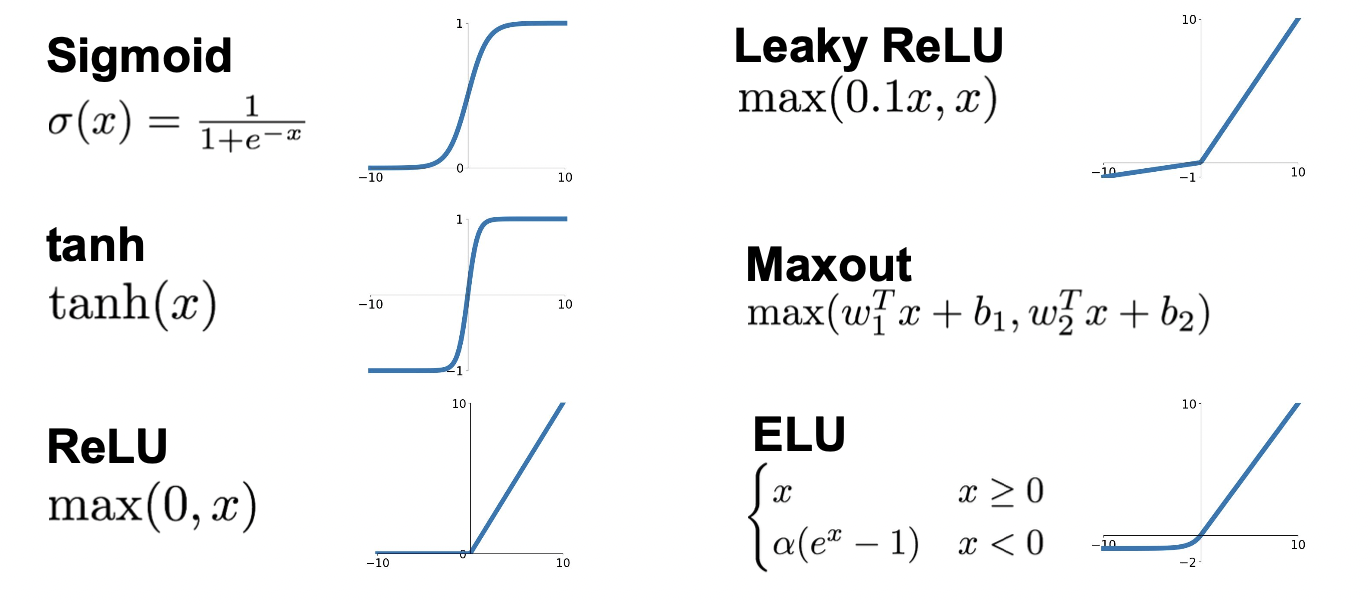
\includegraphics[width=.95\linewidth]{prev_activation.png}
	\end{center}
\end{frame}


%\begin{frame}{В предыдущих сериях: инициализация} 
%	\begin{center}
%		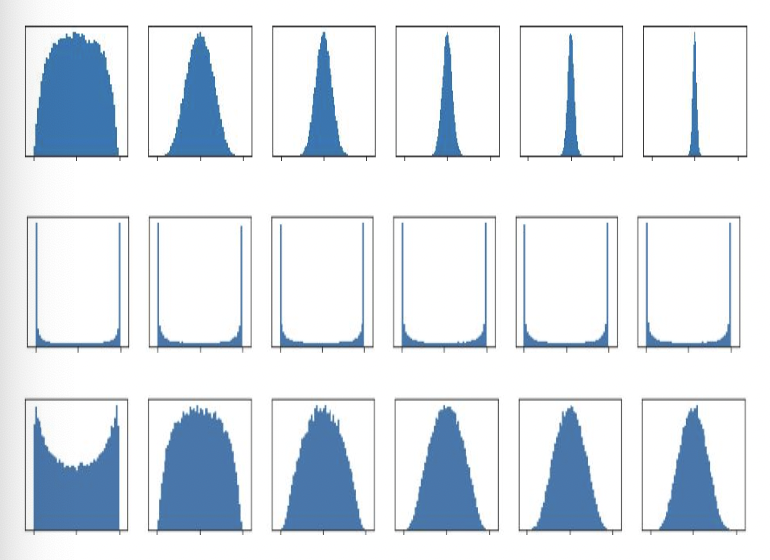
\includegraphics[width=.7\linewidth]{prev_init.png}
%	\end{center}
%\end{frame}

\begin{frame}{В предыдущих сериях: предобработка} 
	\begin{center}
		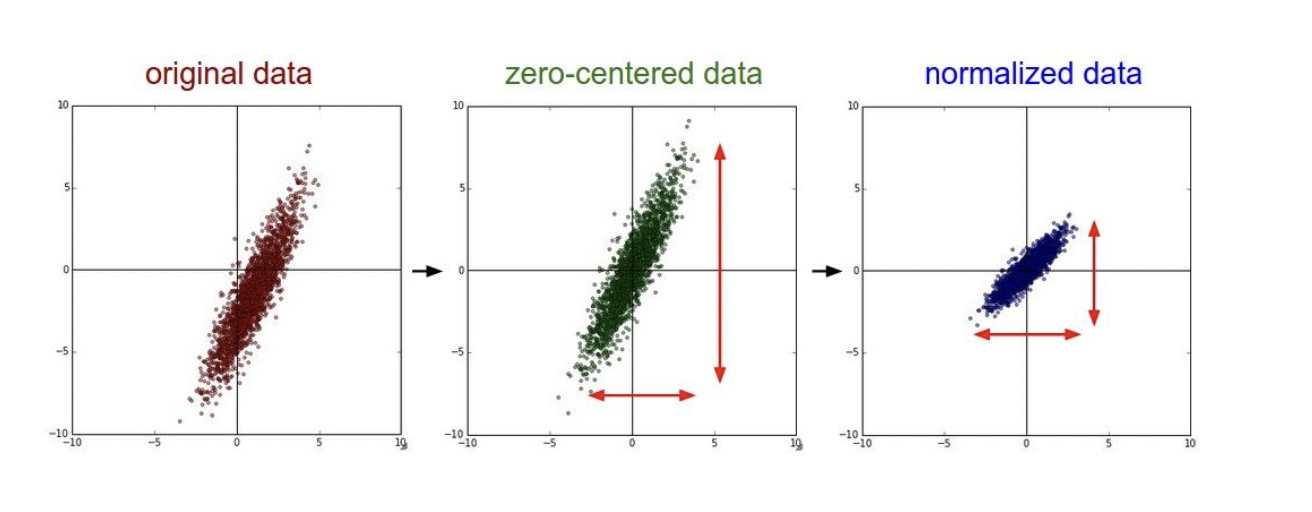
\includegraphics[width=.9\linewidth]{prev_prep.png}
	\end{center}
\end{frame}

%\begin{frame}{В предыдущих сериях: регуляризация} 
%	\begin{center}
%		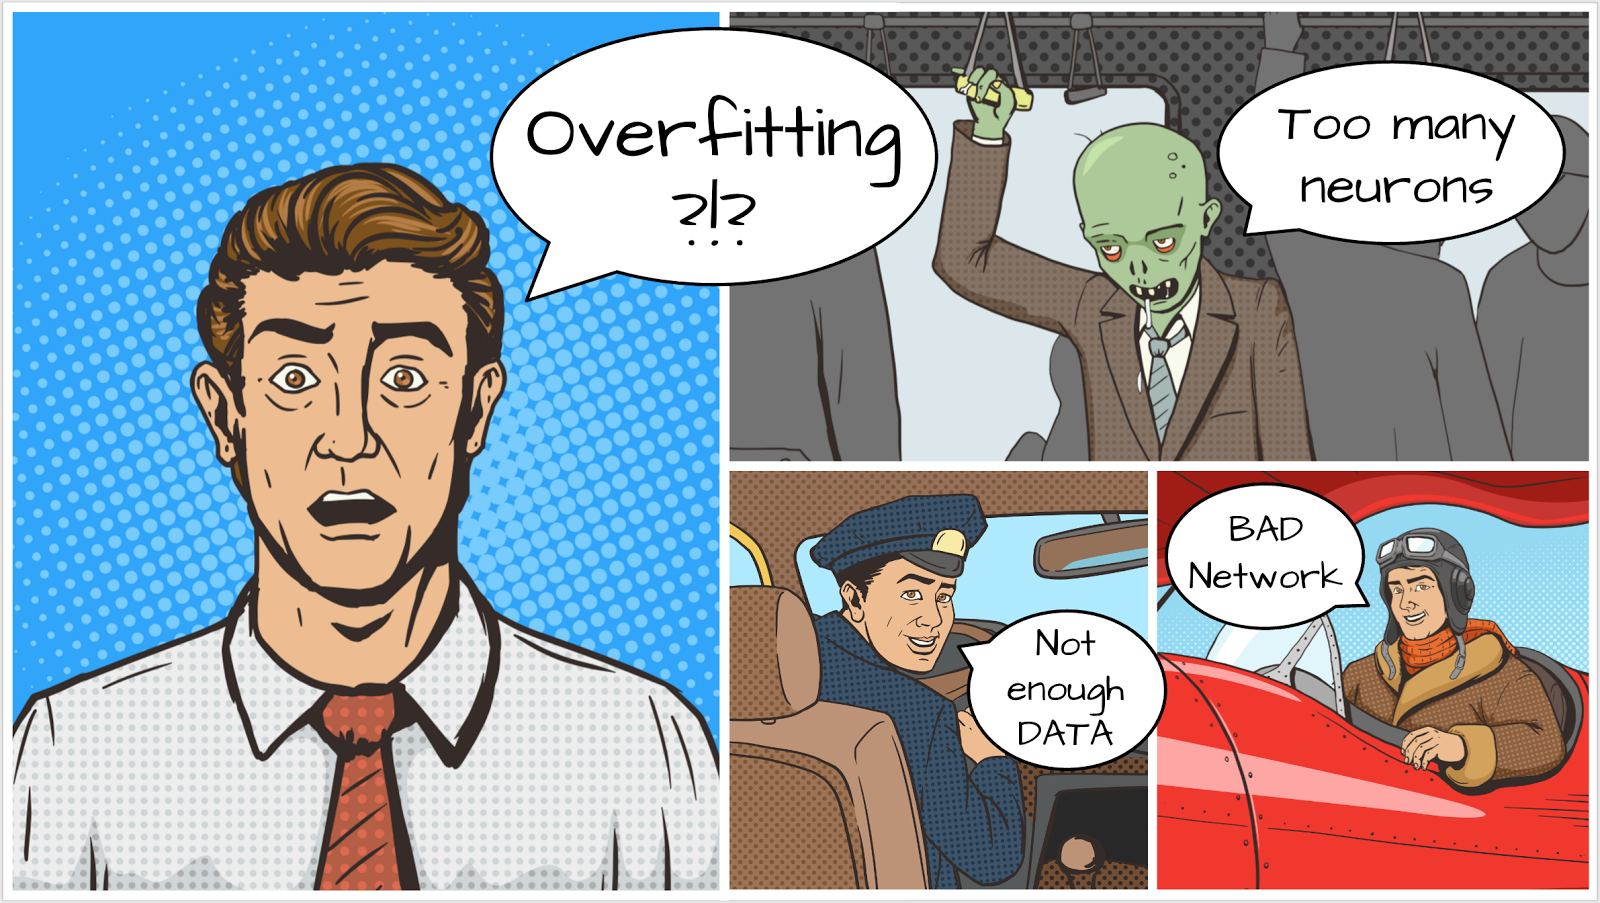
\includegraphics[width=.9\linewidth]{prev_overfitting.png}
%	\end{center}
%\end{frame}

\begin{frame}{В предыдущих сериях: 50 оттенков градиентного спуска} 
	\begin{center}
		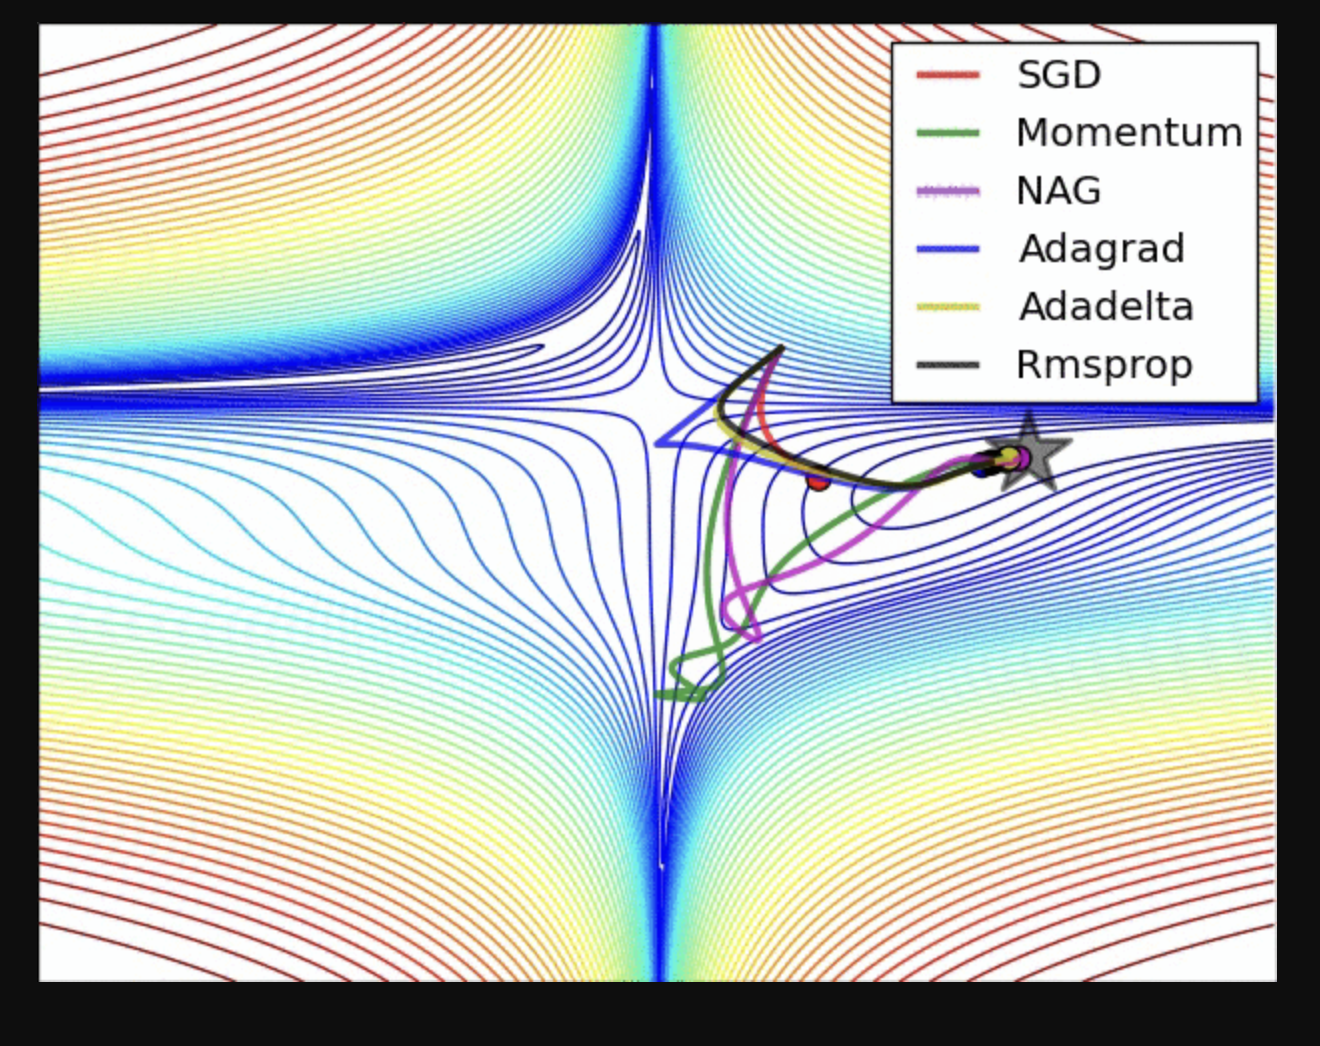
\includegraphics[width=.55\linewidth]{prev_grad.png}
	\end{center}
\end{frame}


\begin{frame}{Agenda}
\begin{wideitemize}
	\item Переобучение нейронных сетей
	\item Дропаут и рання остановка
	\item Регуляризация и weight decay
	\item Learning rate (LR) scheduling
		
	\item Инициализация весов 
	\item Нормализация по батчам 
	
	\item Организация DL-экспериментов 
\end{wideitemize} 
\end{frame}


\begin{transitionframe}
	\begin{center}
		\Huge Переобучение нейронных сетей
	\end{center}
	\centering 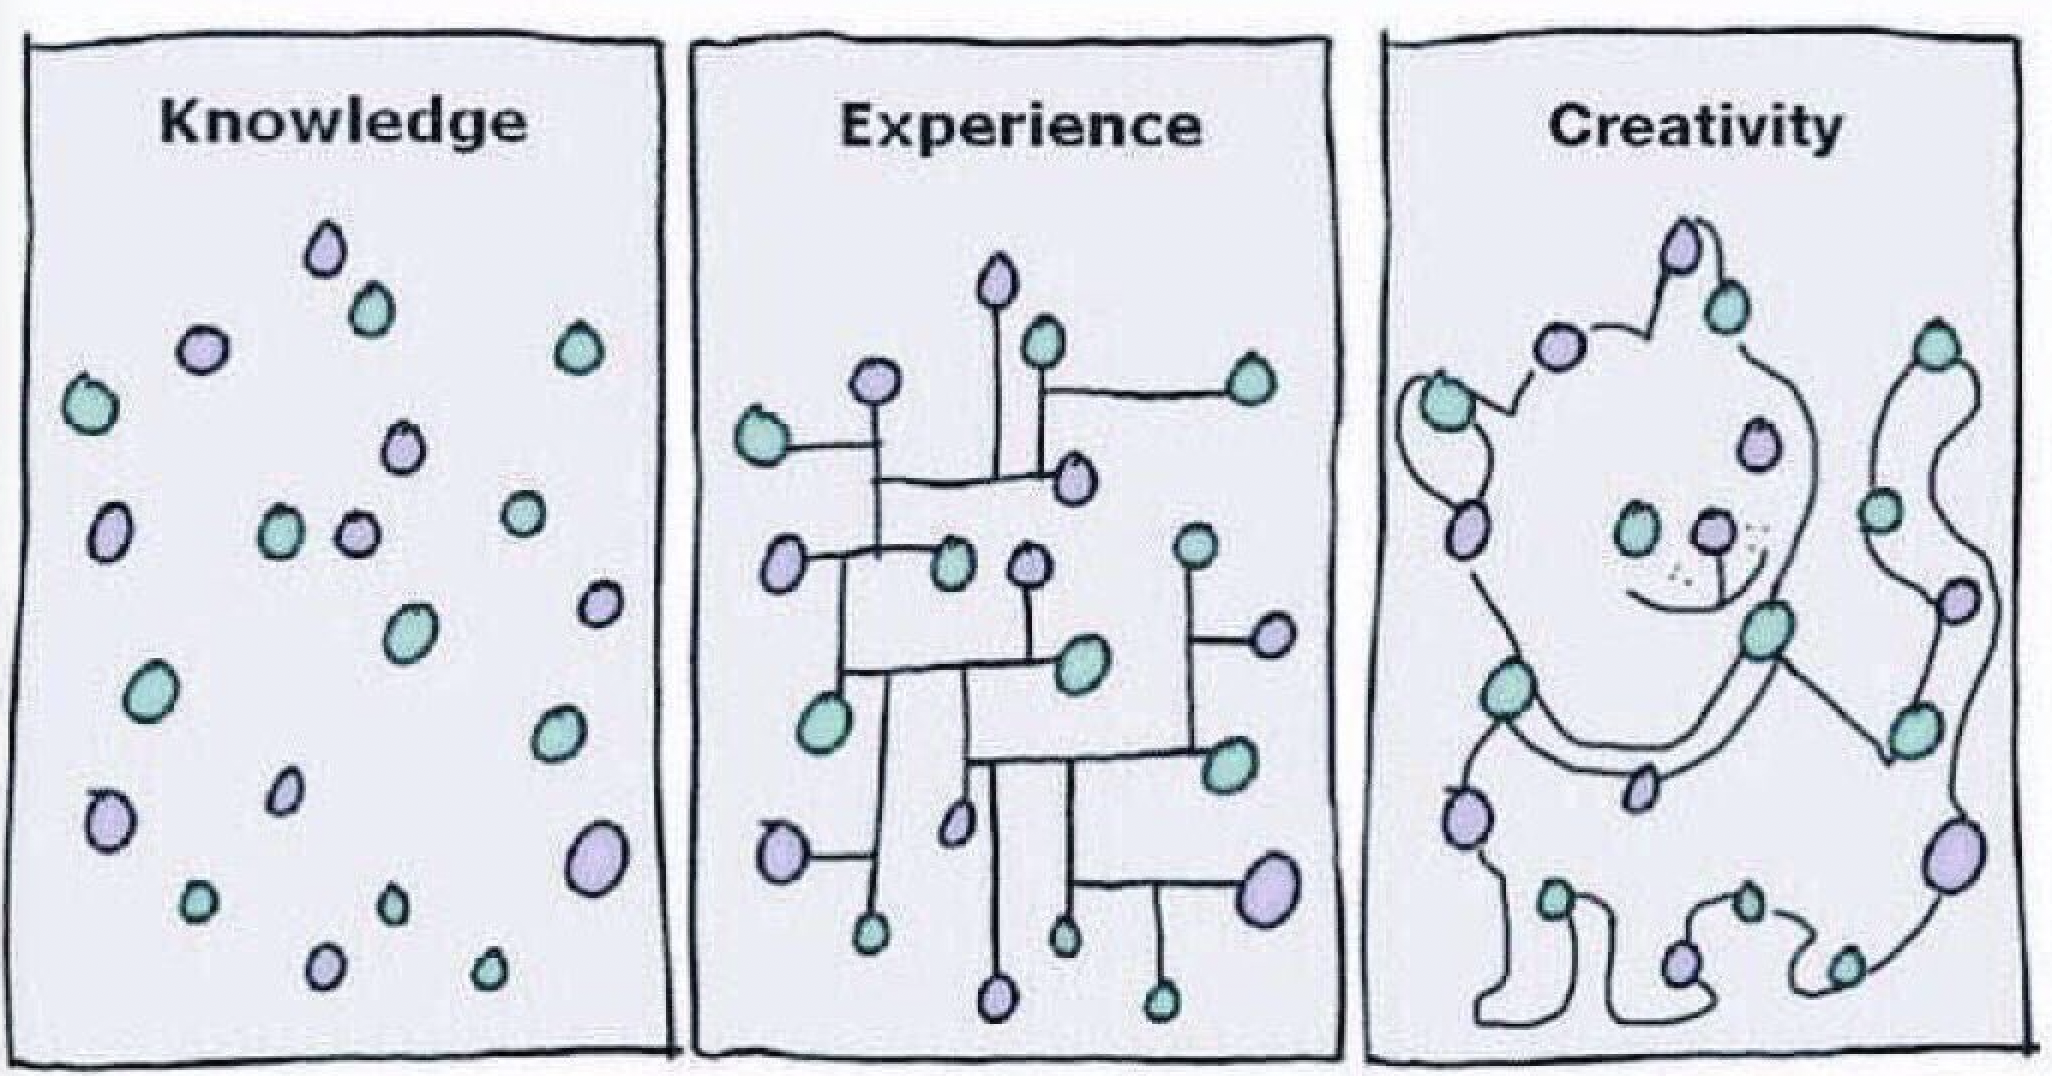
\includegraphics[scale = 0.2]{over.png}
\end{transitionframe}


\begin{frame}{Что такое асимптотика?}
	\begin{wideitemize}
		\item $n$ — число наблюдений  \only<3-4>{$k$ — число параметров}
		\item Обучение почти любой ML-модели  — максимизация правдоподобия 
		\item \only<1>{ При $n \to \infty$ модель работает хорошо} \only<2-4>{\sout{При $n \to \infty$ модель работает хорошо}}
		\only<3-4>{\item \alert{При $\frac{n}{k} \to \infty$ модель работает хорошо}}
		\only<4>{\item Мы живём в эпоху перепараметризованных моделей, $k$~сильно~больше~$n$ }
		\only<4>{\item У таких моделей вскрывается много интересных свойств  [1]}
	\end{wideitemize}
	\only<4>{\vfill %
		\footnotesize 
		\color{blue} [1] \url{https://www.youtube.com/watch?v=SKYXBPCJHCg&t}}
\end{frame}


{
	\usebackgroundtemplate{ 
		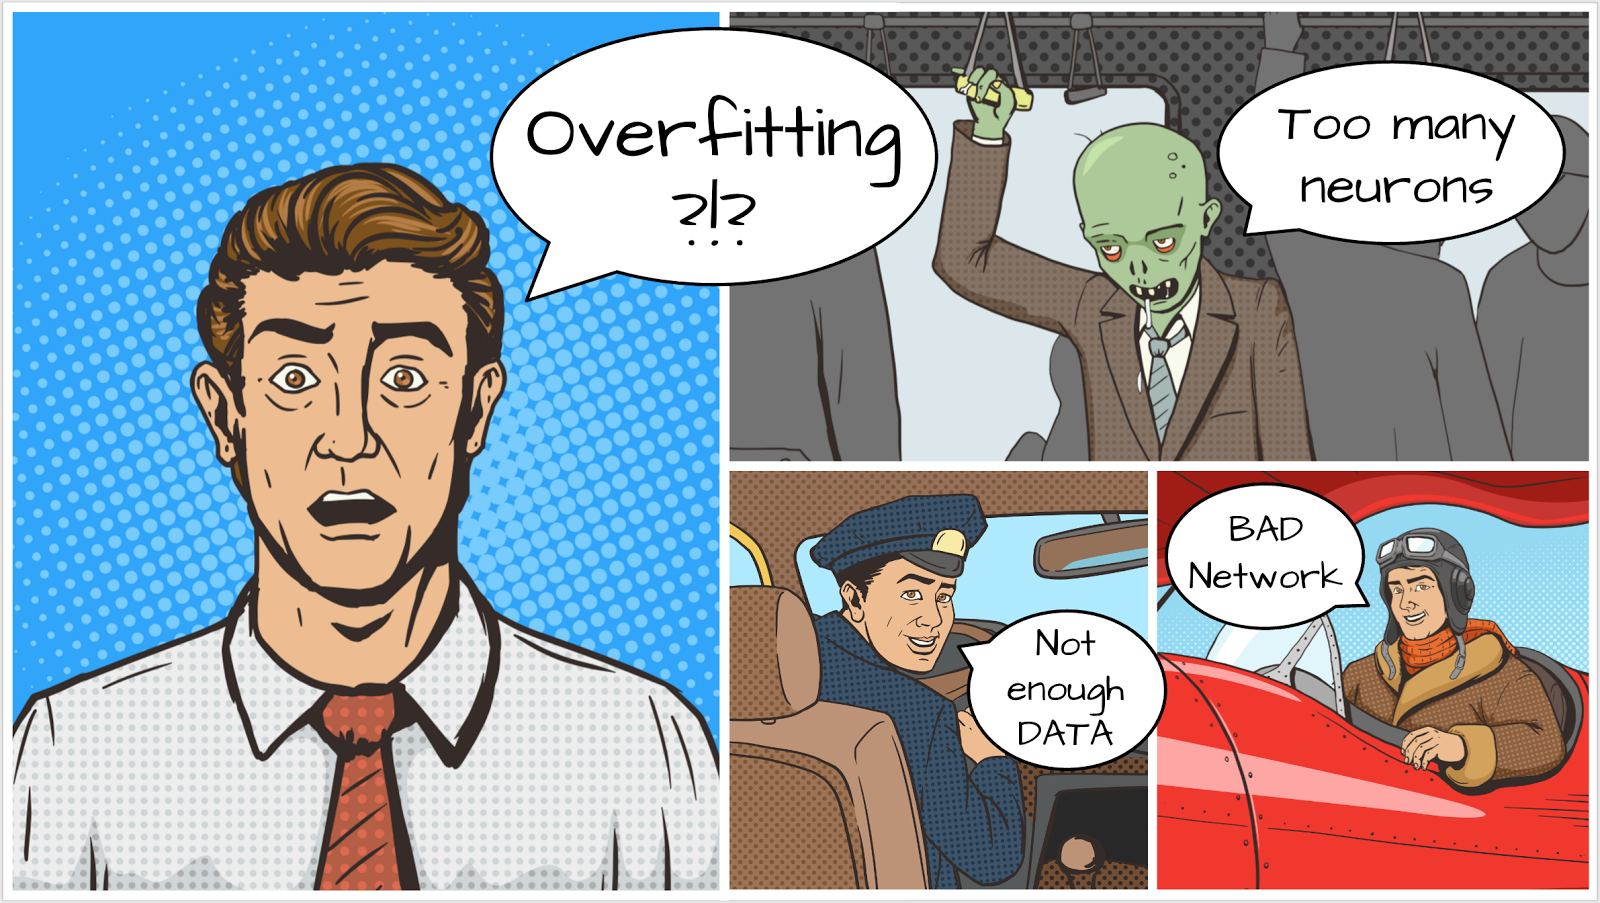
\includegraphics[width=\paperwidth]{overfitting.png}}
	\begin{frame}
	\end{frame}
}

\begin{frame}{Размеры сеток и переобучение}
	\begin{center}
		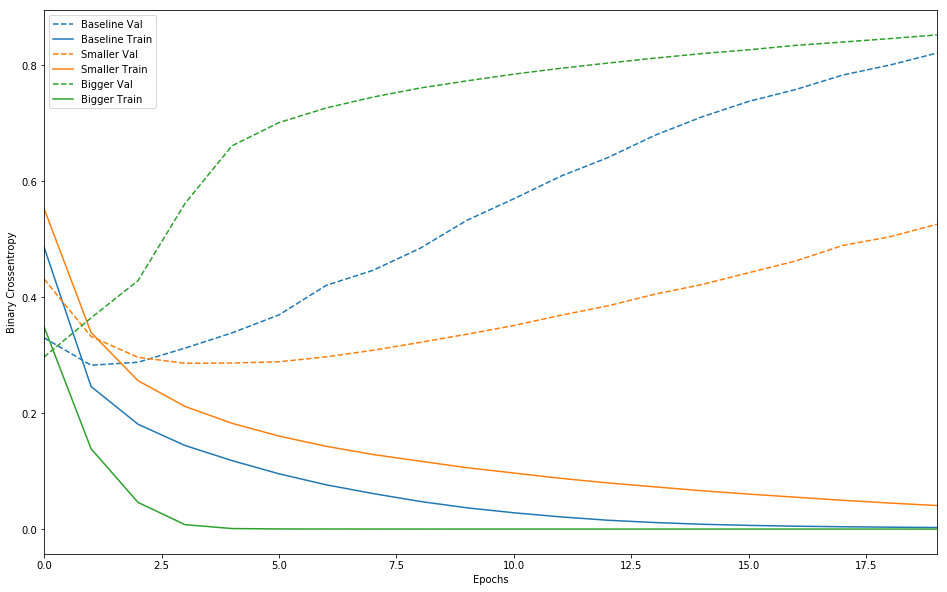
\includegraphics[width=0.7\paperwidth]{big_base_small_fit.png}
	\end{center}
\end{frame}


\begin{frame}{Борьба с переобучением}
	\begin{wideitemize}
		\item Граница сильно размыта
		\item Сокращение числа параметров, изобретение более эффективных архитектур
		\item Регуляризация, разные способы мешать модели подгоняться под обучающую выборку
		\item Более эффективные методы оптимизации
	\end{wideitemize}
\end{frame}


\begin{frame}{Регуляризация}
	\begin{wideitemize}
		\item Любой дополнительный шум в данных — регуляризация
				
		\item $L_2$: приплюсовываем к функции потерь $\lambda \cdot \sum w_i^2$
		
		\item $L_1$: приплюсовываем к функции потерь $\lambda \cdot \sum |w_i|$
		
		\item Вместо классической регуляризации обычно используют weight decay
	\end{wideitemize}
\end{frame}


\begin{frame}{Ранняя остановка (early stopping)}
	\begin{center}
		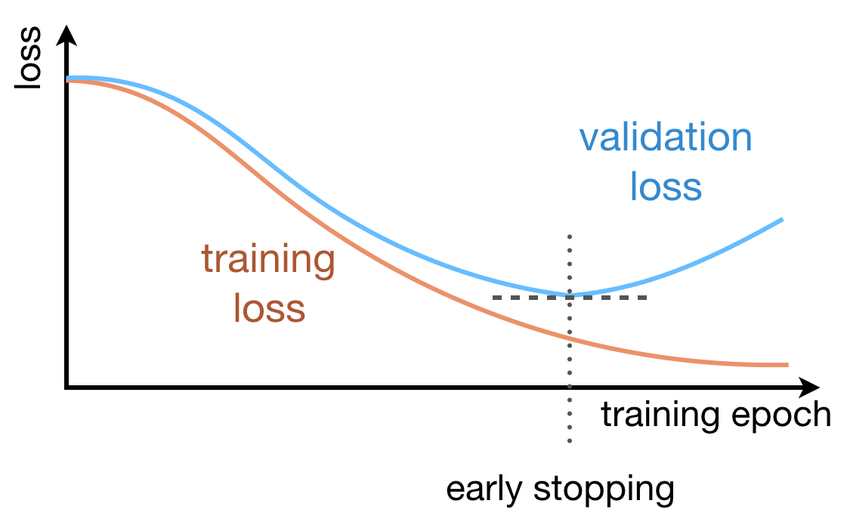
\includegraphics[width=.7\linewidth]{early_stopping.png}
	\end{center}
\end{frame}


\begin{frame}{Ранняя остановка (early stopping)}
	\begin{wideitemize}
		\item  Будем останавливать обучение, когда качество на валидации начинает падать
		\item  Ранняя остановка действует примерно также, как регуляризаторы 
		\item  Например, в книге  Гудфеллоу "Глубокое обучение" на стр. 218 можно найти, что ранняя остановка для линейных моделей эквивалентна $l_2$ регуляризации с MSE, обучаемой SGD
	\end{wideitemize}
\end{frame}


\begin{frame}{Ругуляризация и Dropout}
	\begin{wideitemize}
		\item На практике обычно используют Dropout
		
		\item Он работает похожим на регуляризаторы образом
		
		\item Например, в [1] написано: \\ \mbox{   } \\
		
		\texttt{«We show that the dropout regularizer is first-order equivalent to an L2 regularizer applied after scaling the features by an estimate of the inverse diagonal Fisher information matrix»}
	\end{wideitemize}
	\vfill %
	\footnotesize 
	\color{blue} [1] \url{https://arxiv.org/abs/1307.1493} 
\end{frame}


\begin{transitionframe}
	\begin{center}
		 \Huge Weight decay \\
	\centering 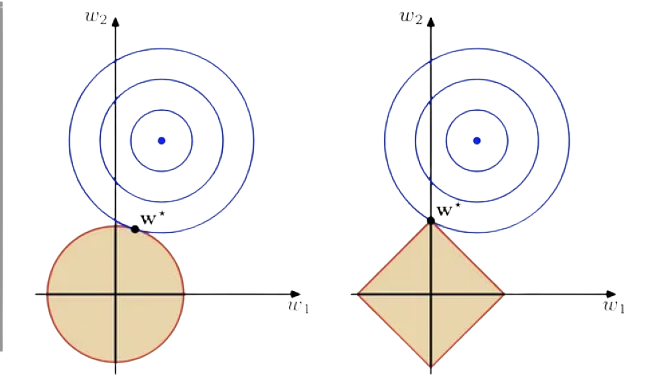
\includegraphics[scale = 0.35]{reg.png}
	\end{center}
\end{transitionframe}


\begin{frame}{Momentum SGD}
		$$
		Q_\lambda(w) = \frac{1}{n} \cdot \sum\limits_{i=1}^{n} L_i(w) + \frac{1}{2}\lambda \cdot ||w||^2_2
		$$
			
			
		$$
		\begin{cases}
			g_t = \nabla_w Q(w_{t-1}) + \lambda \cdot w_{t-1} \\
			m_t = \mu \cdot m_{t-1} + g_t\\
			w_t = w_{t-1} - \eta_t \cdot m_t \\
		\end{cases}
		$$
		
		Подставим первую строку во вторую, а вторую в третью:
		
		\begin{multline*}
			w_t = w_{t-1} - \eta_t \cdot (\mu \cdot m_{t-1} + \nabla_w Q(w_{t-1}) + \lambda \cdot w_{t-1}) = \\ =\alert{\underbrace{(1-\eta_t\cdot \lambda)}_{<1}}\cdot w_{t-1} - \eta_t\cdot(\mu\cdot m_{t-1} + \nabla_wQ(w_{t-1}))
		\end{multline*}
\end{frame}


\begin{frame}{Weight decay для momentum SGD}

	\begin{wideitemize}
		\item  мы шагаем по старому градиенту (без регуляризатора), но из новых весов
		
		$$
			w_t = \alert{\underbrace{(1-\eta_t\cdot \lambda)}_{<1}}\cdot w_{t-1} - \eta_t\cdot(\mu\cdot m_{t-1} + \nabla_wQ(w_{t-1}))
		$$
		
		\item $\lambda$   — weight decay
		
		\item  типичные значения $\lambda$ для нейронок:  $1e-4, 1e-5$
	\end{wideitemize}
\end{frame}


\begin{frame}{Adam}
	$$
		Q_\lambda(w) = \frac{1}{n} \cdot \sum\limits_{i=1}^{n} L_i(w) + \frac{1}{2}\lambda \cdot ||w||^2_2
	$$	

	$$
		\begin{cases}
			g_t = \nabla_w Q(w_{t-1}) + \lambda \cdot w_{t-1} \\
			m_t = \beta_1 \cdot m_{t-1} + (1-\beta_1) \cdot g_t \\
			v_t = \beta_2 \cdot v_{t-1} + (1-\beta_2) \cdot g_t^2\\
			\hat{m}_t = \frac{1}{1-\beta_1^t} \cdot m_t \\
			\hat{v}_t = \frac{1}{1-\beta_2^t}v_t \\
			w_t = w_{t-1} -\eta_t \cdot \frac{\hat{m}_t}{\sqrt{\hat{v}_t} + \varepsilon}
		\end{cases}
	$$
	
	Гиперпарметры от авторов (обычно их не меняют):
	
	$$
	\beta_1 = 0.9, \beta_2 = 0.999 
	$$
	
\end{frame}


\begin{frame}{Adam}
	\begin{multline*}
		w_t = w_{t-1} - \eta_t \cdot \frac{m_t}{1-\beta_1^t} \cdot \frac{1}{\sqrt{\hat{v}_t} + \varepsilon} = \\ = w_t = w_{t-1} - \eta_t \cdot \frac{\beta_1 \cdot m_{t-1} + (1-\beta_1) \cdot g_t}{1-\beta_1^t} \cdot \frac{1}{\sqrt{\hat{v}_t} + \varepsilon} = \\ =w_t = w_{t-1} - \eta_t \cdot \frac{\beta_1 \cdot m_{t-1} + (1-\beta_1) \cdot (\nabla_w Q(w_{t-1}) + \lambda \cdot w_{t-1})}{1-\beta_1^t} \cdot \frac{1}{\sqrt{\hat{v}_t} + \varepsilon} =\\=w_{t-1}\cdot \left(\underbrace{1}_{\text{вектор единиц}} - \frac{\eta_t \cdot \lambda\cdot (1-\beta_1)}{1-\beta_1^t} \cdot \alert{\frac{1}{\sqrt{\hat{v}_t}+\varepsilon}}\right) -\dots
		\end{multline*}
	
\alert{Регуляризация работает по-разному — веса штрафуются по-разному, мы хотели от регуляризации не этого!}
\end{frame}


\begin{frame}{AdamW}

Это модификация Adam, в которой мы делаем честный weight decay, из-за этого сетка должна меньше переобучаться

$$
\begin{cases}
	g_t = \nabla_w Q(w_{t-1}) \\
	m_t = \beta_1 \cdot m_{t-1} + (1-\beta_1) \cdot g_t \\
	v_t = \beta_2 \cdot v_{t-1} + (1-\beta_2) \cdot g_t^2\\
	\hat{m}_t = \frac{1}{1-\beta_1^t} \cdot m_t \\
	\hat{v}_t = \frac{1}{1-\beta_2^t}v_t \\
	w_t = (1-\eta_t\cdot\lambda)\cdot w_{t-1} -\eta_t \cdot \frac{\hat{m}_t}{\sqrt{\hat{v}_t} + \varepsilon}
\end{cases}
$$

\vfill %
\footnotesize 
\color{blue} \url{https://arxiv.org/pdf/1711.05101.pdf}
\end{frame}


\begin{transitionframe}
	\begin{center}
		\Huge Ландшафт функции потерь
	\end{center}
	\centering 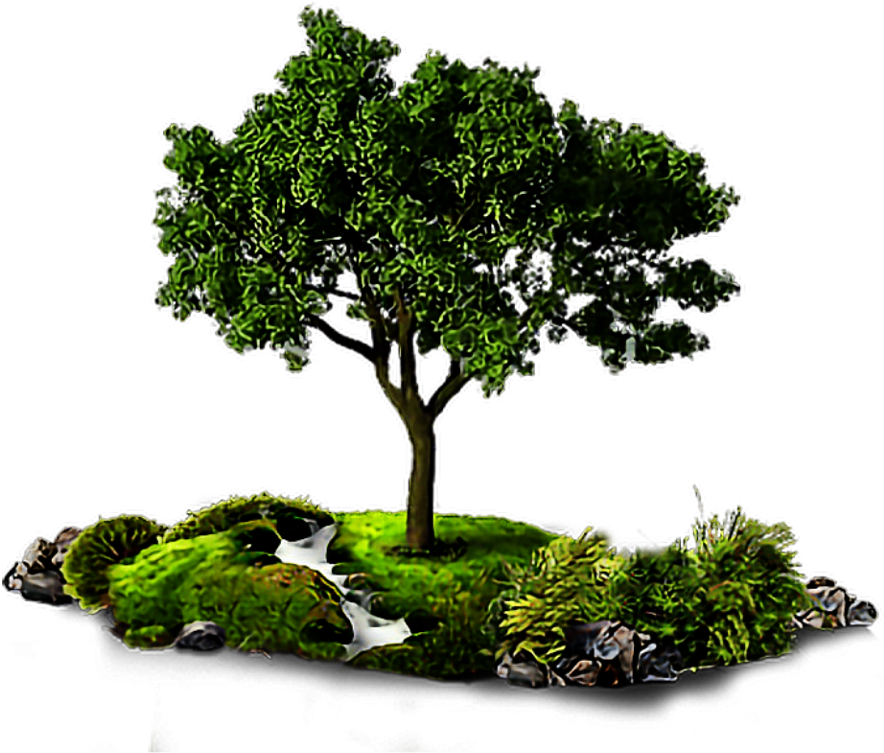
\includegraphics[scale = 0.1]{land.png}
\end{transitionframe}


\begin{frame}{Боб чилит в локальном минимуме}
	\begin{center}
		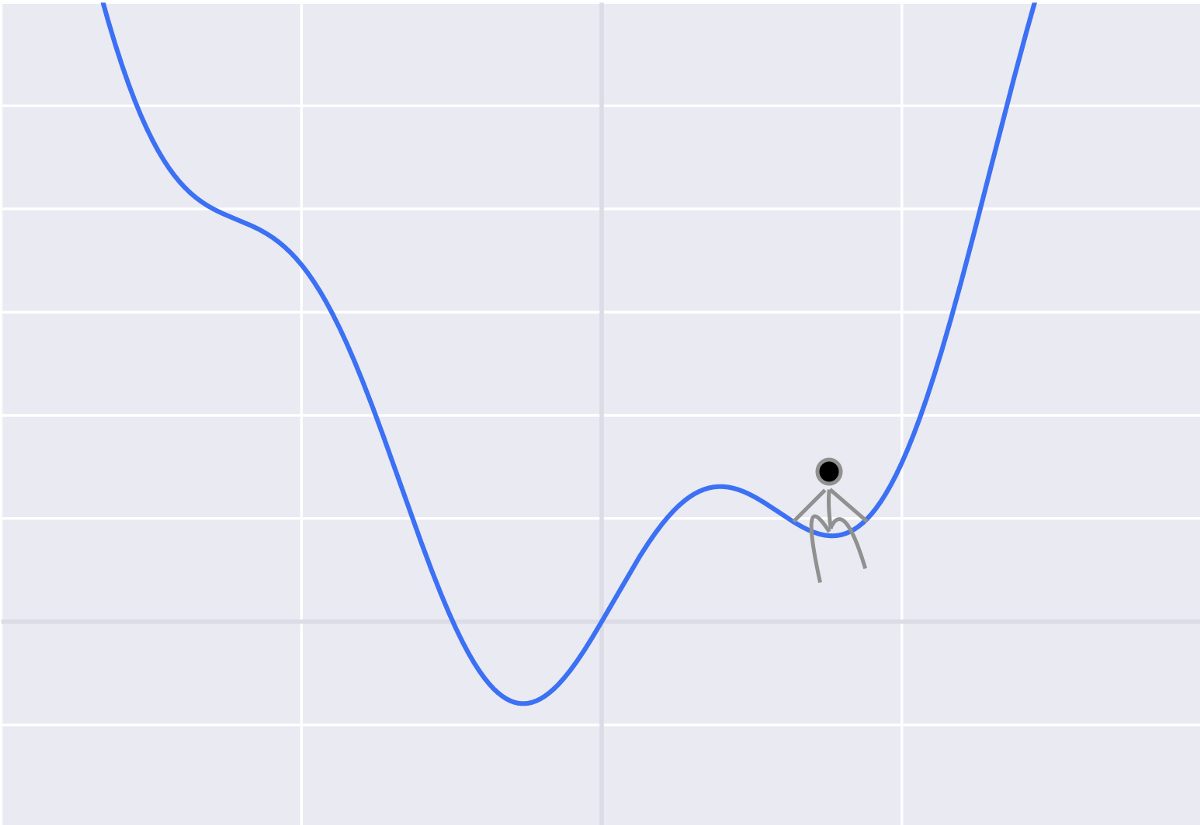
\includegraphics[width=0.6\paperwidth]{bob_local_chill.png}
	\end{center}
	\vfill %
	\footnotesize 
	\color{blue} \url{https://hackernoon.com/life-is-gradient-descent-880c60ac1be8}
\end{frame}


\begin{frame}{Седловые точки}
	\begin{center}
		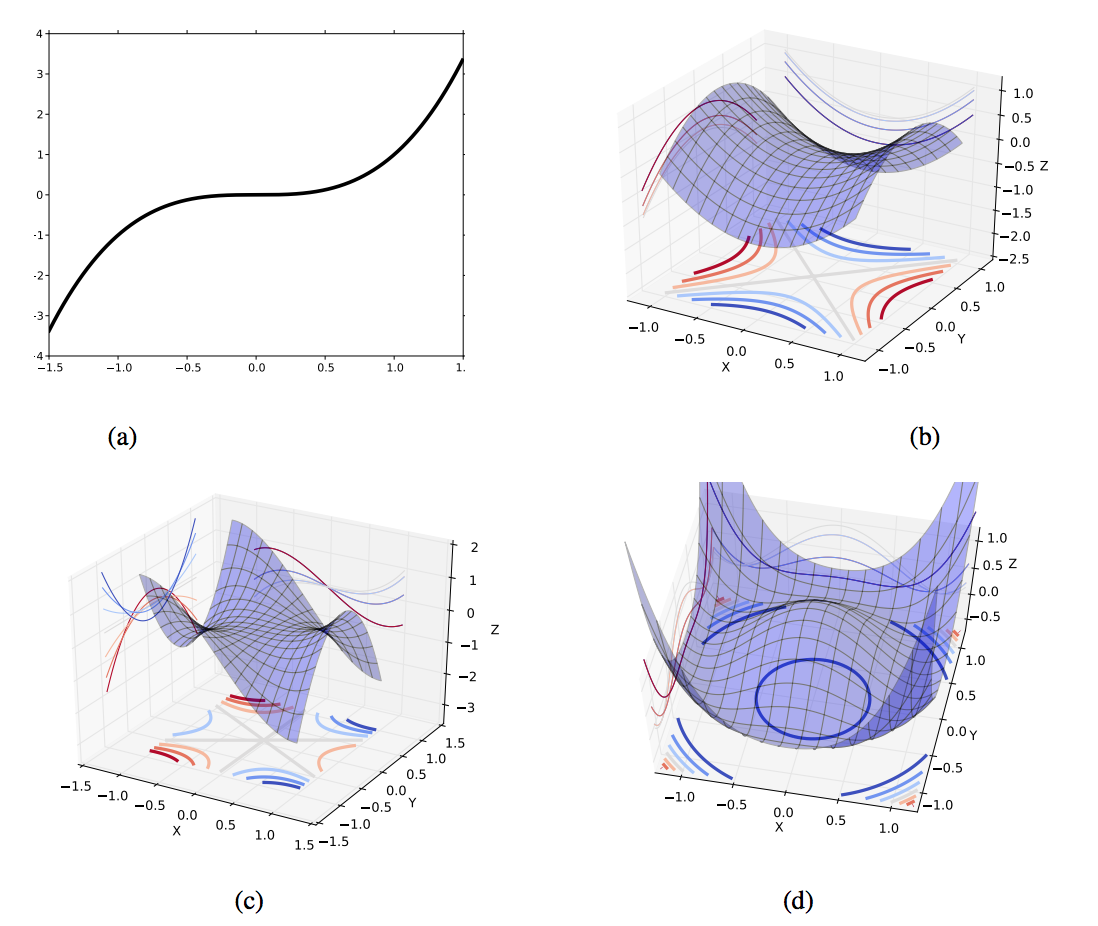
\includegraphics[width=0.5\paperwidth]{sedlo.png}
	\end{center}
	\vfill %
	\footnotesize 
	\color{blue} \url{https://arxiv.org/pdf/1406.2572.pdf}
\end{frame}


\begin{frame}{Визуализация потерь}
	\begin{center}
		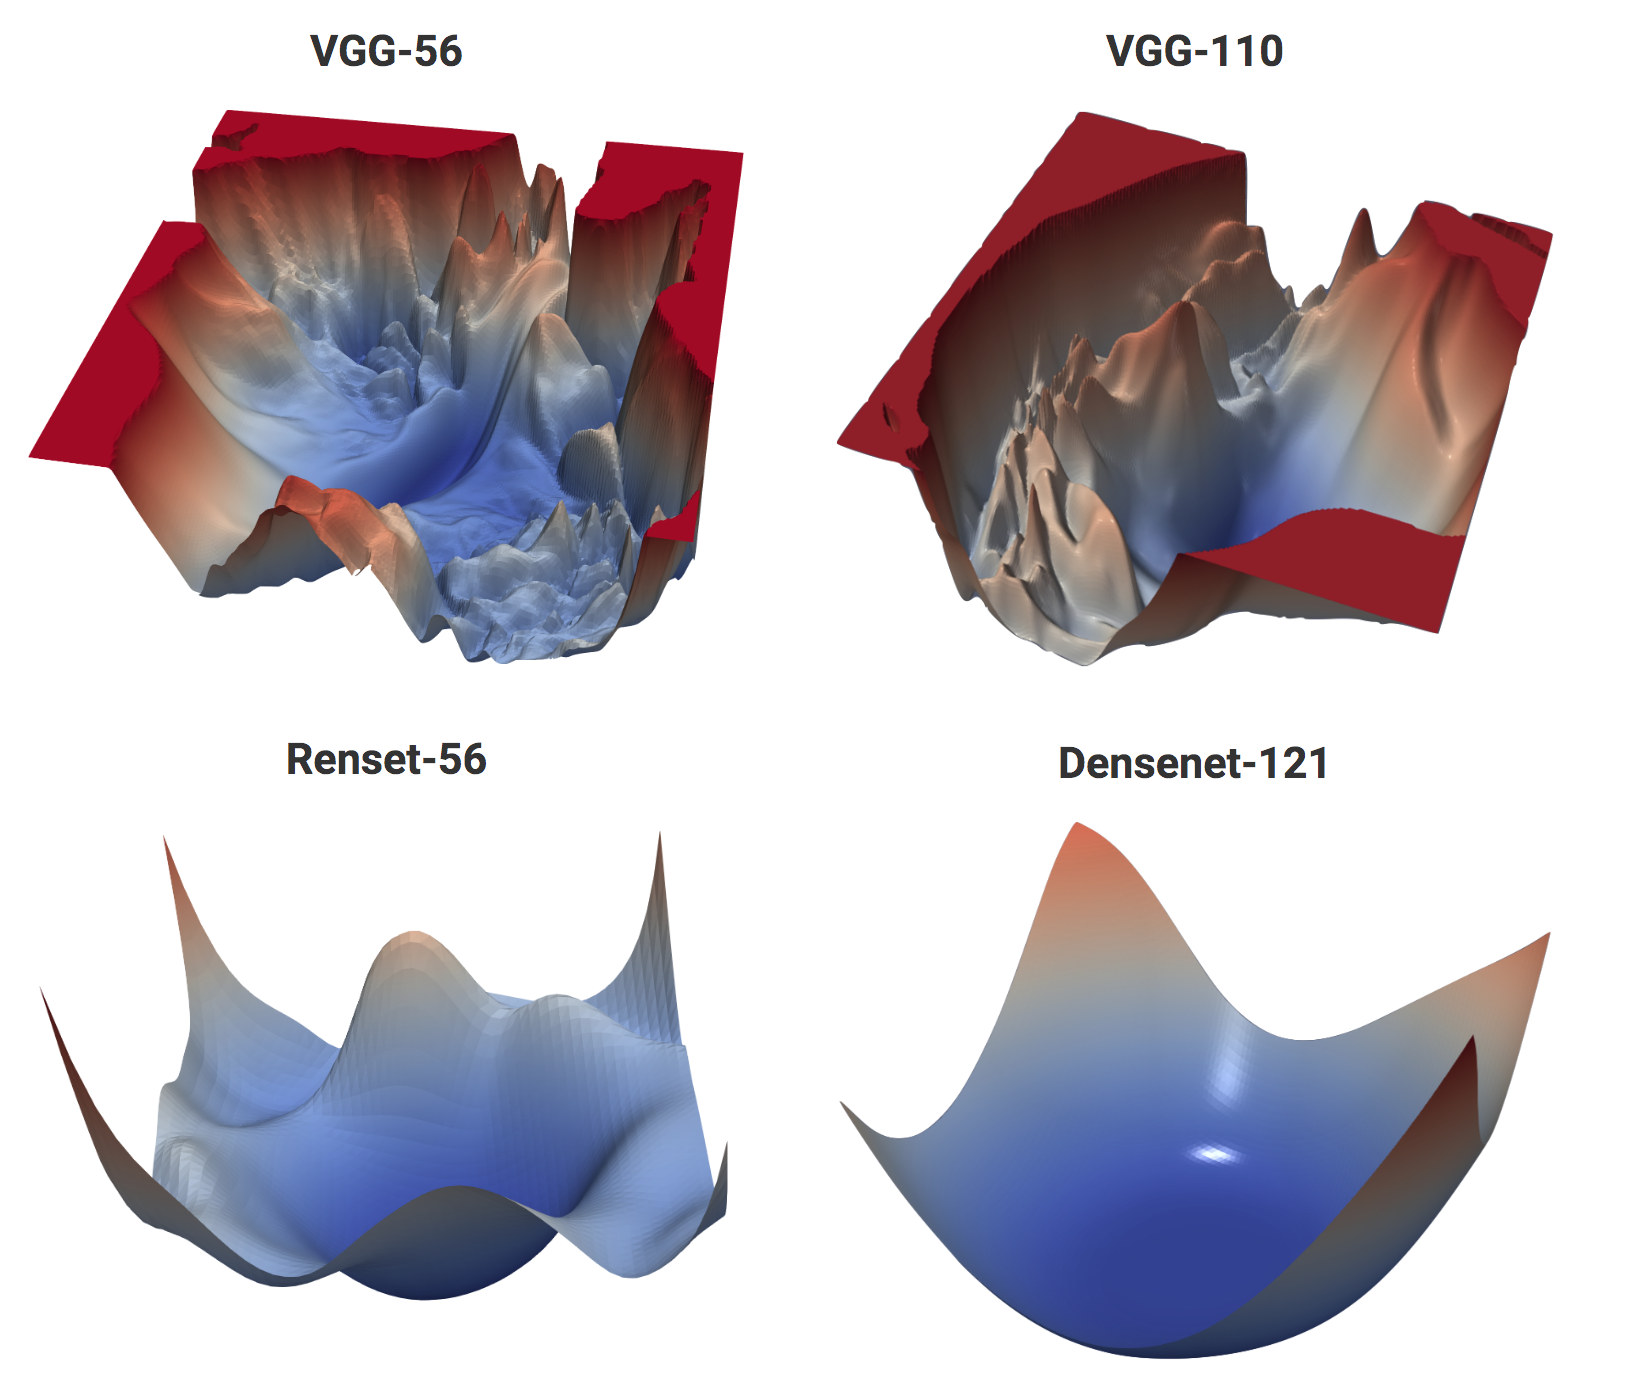
\includegraphics[width=0.5\paperwidth]{loss.png}
	\end{center}
	\vfill %
	\footnotesize 
	\color{blue} \url{https://arxiv.org/pdf/1712.09913.pdf} \newline  \url{https://github.com/tomgoldstein/loss-landscape}
\end{frame}


\begin{frame}{LR scheduling}
	\begin{wideitemize}
		\item Процедура изменения learning rate по какому-то правилу
		\item LR во время обучения всегда надо изменять (теряем проценты в качестве)
	\end{wideitemize}
	\begin{center}
		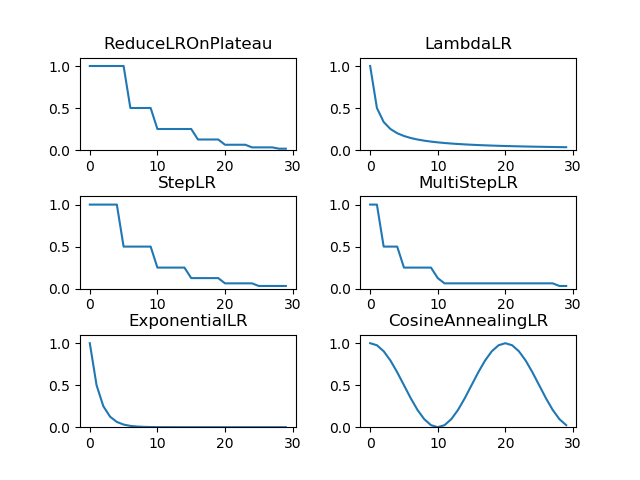
\includegraphics[width=0.5\paperwidth]{lr_sheduling.png}
	\end{center}
\end{frame}


\begin{frame}{Циклическая скорость обучения (CLR)}
	\begin{wideitemize}
		\item Хочется, чтобы был шанс вылезти из локального минимума, а также шанс сползти с седла $\Rightarrow$ давайте менять глобальную скорость обучения циклически
	\end{wideitemize}
	\begin{center}
		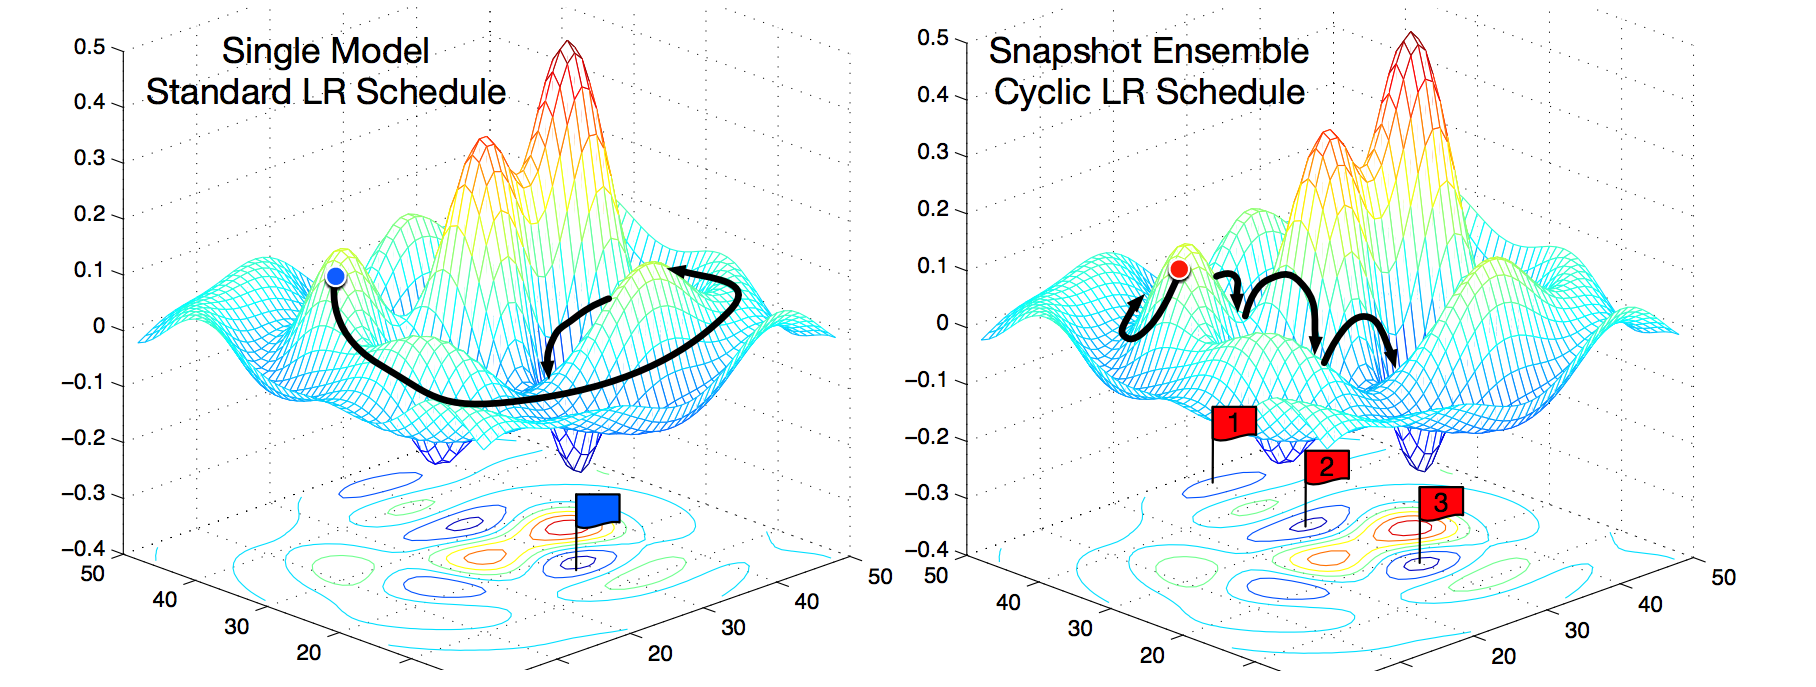
\includegraphics[width=0.75\paperwidth]{cycle_sgd.png}
	\end{center}
\end{frame}


\begin{frame}{Циклическая скорость обучения (CLR)}
	\begin{columns}[T] % align columns
		\begin{column}{.48\textwidth}
			\centering 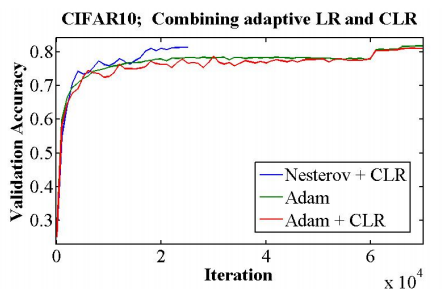
\includegraphics[scale=0.55]{cycle_2.png}
		\end{column}%
		\hfill%
		\begin{column}{.48\textwidth}
			\centering 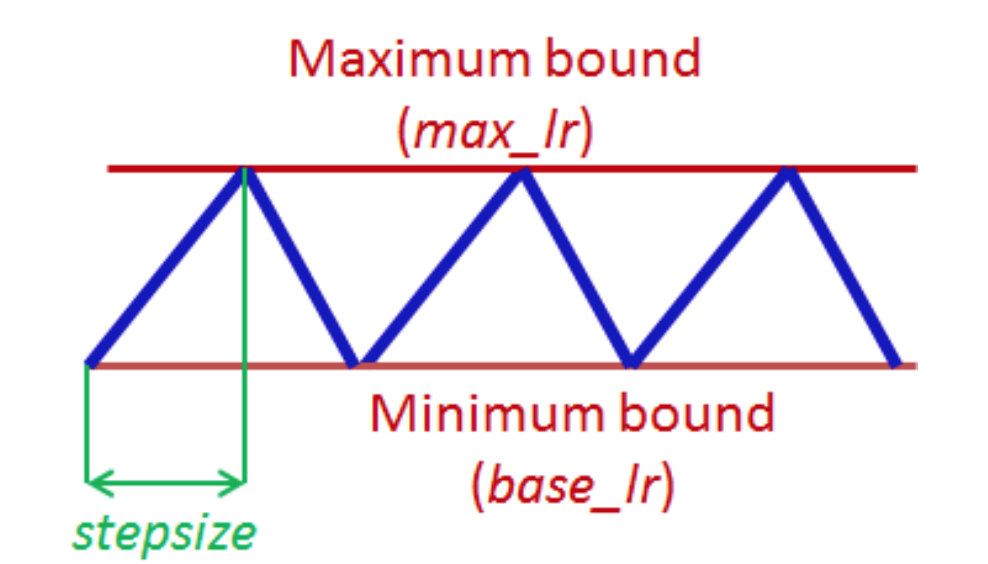
\includegraphics[scale=0.17]{cycle.png} \\ \mbox{ } \\
			Нестеров с CLR отработал \\ быстрее и лучше Adam \\ \alert{Нет одного правильного \\ алгоритма на все случаи}  \\ Всегда надо экспериментировать
		\end{column}%
	\end{columns}
	
	\vfill %
	\footnotesize  
	\color{blue} \url{https://arxiv.org/pdf/1506.01186.pdf} \newline  \url{https://openreview.net/pdf?id=BJYwwY9ll}
\end{frame}


\begin{frame}{LRFinder}
	\begin{wideitemize}
		\item   Эвристика для подбора стартового значения learning rate 
		
		\item  Увеличиваем learning rate после каждого батча, остановка перед взрывом значений loss-функции
		
		\item  Есть готовые реализации (в том числе в pytorch и tensorflow) 
		
		\item  Аналогично можно искать оптимальное значение для momentum
	\end{wideitemize}
	\vfill
	
	\footnotesize
	{\color{blue} \url{https://sgugger.github.io/how-do-you-find-a-good-learning-rate.html} \newline 
		\url{https://arxiv.org/abs/1506.01186} \newline 
		\url{https://arxiv.org/abs/1803.09820}}
\end{frame}




\begin{transitionframe}
	\begin{center}
		% \Huge Dropout  
		
\includegraphics[scale = 0.25]{dropout_beer.png}
	\end{center}
\end{transitionframe}


% Оформить слайд как цитату, мб впихнуть фотку Хинтона
\begin{frame}{Хинтон и банк}
	
	Посещая свой банк я заметил, что операционисты, обслуживающие меня, часто меняются. Я спросил одного из них, почему так происходит. Он сказал, что не знает, но им часто приходится переходить с места на место. Я предположил, что это делается для исключения мошеннического сговора с сотрудником банка. 
	
	\par \mbox{ } \par 
	
	Это навело меня на мысль, что \alert{удаление случайно выбранного подмножества нейронов}  из каждого примера может помочь \alert{предотвратить заговор модели с исходными данными} и ослабить эффект переобучения. 
	
	\par \mbox{ } \par 
	
	\vfill %
	\footnotesize
	{\color{blue} \url{https://www.reddit.com/r/MachineLearning/comments/4w6tsv/ama_we_are_the_google_brain_team_wed_love_to}}
\end{frame}


\begin{frame}{Dropout}
	\begin{wideitemize}	
		\item При каждом прямом проходе мы зануляем выход нейрона с вероятностью $p$ 
		\item Делает нейроны более устойчивыми к случайным возмущениям
	\end{wideitemize}
	
	\begin{center}
		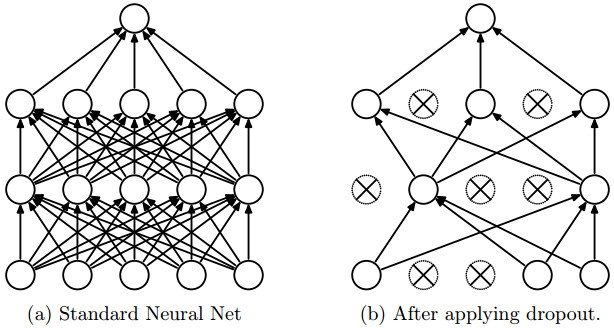
\includegraphics[width=0.5\paperwidth]{dropout2.png}
	\end{center}
	
	\vfill %
	\footnotesize
	{\color{blue} \url{http://www.cs.toronto.edu/~rsalakhu/papers/srivastava14a.pdf}}
\end{frame}


\begin{frame}{Dropout}
	\begin{wideitemize}	
		\item Борьба с ко-адоптацией, не все соседи похожи  друг на друга, не все дети похожи  на родителей
		\item  Dropout эквивалентен обучению ансамбля из $2^n$ сетей
	\end{wideitemize}
	
	\begin{center}
		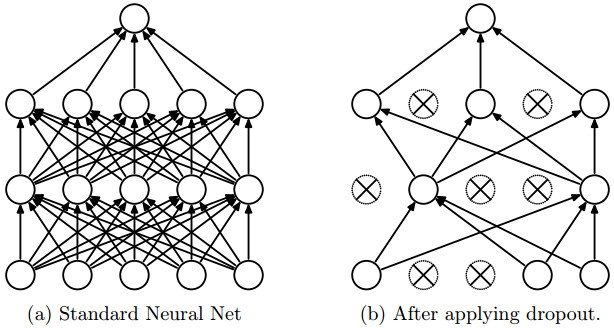
\includegraphics[width=0.5\paperwidth]{dropout2.png}
	\end{center}
	
	\vfill %
	\footnotesize
	{\color{blue} \url{http://www.cs.toronto.edu/~rsalakhu/papers/srivastava14a.pdf}}
\end{frame}


\begin{frame}{Dropout в формулах} 
	\begin{wideitemize}
		\item  Можно определить как слой $d(h)$ 
		\item  Параметров у слоя нет, есть только гиперпараметр $p$
		\pause 
		\item  	forward pass без dropout:  \[o = f(XW)\]
		\item  	forward pass с dropout:  \[o = d \cdot f(XW), \quad d = (d_1, \ldots, d_k)  \sim iid \vspace{10mm} Bern(1 - p)\]
		\pause 	
	\end{wideitemize}
	\[
	o_i = d_i \cdot f(w x_i^T) = \begin{cases} f(w x_i^T) , & 1-p \\ 0,  & p \end{cases}
	\]	
	\vfill 
	\alert{Дропаут — это просто небольшая модификация функции активации}
\end{frame}


\begin{frame}{Dropout в формулах} 
	\begin{wideitemize}
		\item forward pass:
		
		\begin{equation*}
			\begin{aligned}
				& o = f(X \cdot W  ) \\
				& \alert{o = d \cdot f(X \cdot W ), \quad  d = (d_1, \ldots, d_k) \sim iid \vspace{10mm} Bern(1 - p)} 
			\end{aligned}
		\end{equation*}
		
		\item backward pass:
		\begin{equation*}
			\begin{aligned}
				& grad = f'(h) \cdot W \cdot grad  \\
				& \alert{ grad =  d \cdot f'(h) \cdot W \cdot grad} 
			\end{aligned}
		\end{equation*}			
	\end{wideitemize}
\end{frame}


\begin{frame}{Dropout}
	\begin{wideitemize}
		\item  При обучении мы домножаем часть выходов на $d_i$, тем самым мы изменяем только часть параметров и нейроны учатся более независимо  \alert{$\Rightarrow$ регуляризация}
		
		\item Дропаут выплёвывает случайные выходы,  \alert{ что делать на стадии тестирования?}
		
		\only<2->{
			\item Нам надо сымитировать работу такого ансамбля: можно отключать по очереди все возможные комбинации нейронов, получить $2^n$ прогнозов и усреднить их }
		
		\only<3->{ \item Но лучше просто брать по дропауту математическое ожидание: 
			
			$$
			o = (1 - p) \cdot f(X \cdot W)
			$$}
	\end{wideitemize}
\end{frame}

\begin{frame}{Dropout на тестовой выборке}
	\begin{wideitemize}
		\item Но лучше просто брать по дропауту математическое ожидание: 
		
		$$
		o =(1 - p) \cdot f(X \cdot W)
		$$
	\end{wideitemize}
	\begin{columns}
		\begin{column}{.25\textwidth}
			\begin{center}
				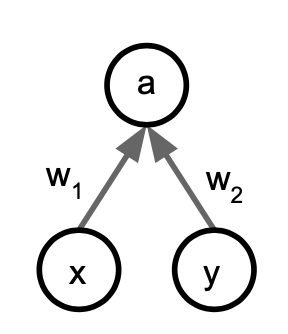
\includegraphics[width=.85\linewidth]{dropout_ex.png}
			\end{center}
		\end{column}
		\begin{column}{.75\textwidth}
			\textbf{Пример:} используем дропаут с вероятностью $0.5$: \\
			\begin{multline*}
				\mathbb{E}(a) = \frac{1}{4} \cdot(w_1 x+ w_2 y) + \frac{1}{4} \cdot(w_1 x+ 0 y) + \\ + \frac{1}{4} \cdot(0 x+ w_2 y) + \frac{1}{4} \cdot(0 x+ 0 y) = \frac{1}{2} \cdot (w_1 \cdot x + w_2 \cdot y)
			\end{multline*}
			\alert{Достаточно домножить выход на $0.5$}
		\end{column}
	\end{columns}
\end{frame}


\begin{frame}{Обратный Dropout}
	\begin{wideitemize}
		\item   На тесте ищем математическое ожидание: 
		\[
		o = (1 - p) \cdot f(X \cdot W )
		\] 
		
		\item \alert{Это неудобно! Надо переписывать функцию для прогнозов!}  \pause
		
		\item Давайте лучше будем домножать на $\frac{1}{1 - p}$ на этапе обучения: 
		
		\begin{equation*}
			\begin{aligned}
				& \text{train: }   \quad o = \frac{1}{1 - p} \cdot d \cdot f(X \cdot W) \\ 
				& \text{test:  }   \quad o = f(X \cdot W ) \\
			\end{aligned}
		\end{equation*}		
	\end{wideitemize}
\end{frame}

\begin{frame}{Интерпретация} 
	\begin{wideitemize}
		\item  Мы обучаем все возможные архитектуры нейросетей, которые получаются из исходной выбрасыванием отдельных нейронов
		\item  У всех этих архитектур общие веса
		\item  На этапе применения усредняем прогнозы всех этих архитектур
	\end{wideitemize}
\end{frame}


\begin{transitionframe}
	\begin{center}
		\Huge  Батч-нормализация
	\end{center}
	\centering 
\includegraphics[scale = 0.25]{batcAlice.png}
\end{transitionframe}


\begin{frame}{Стандартизация}
	\begin{center}
		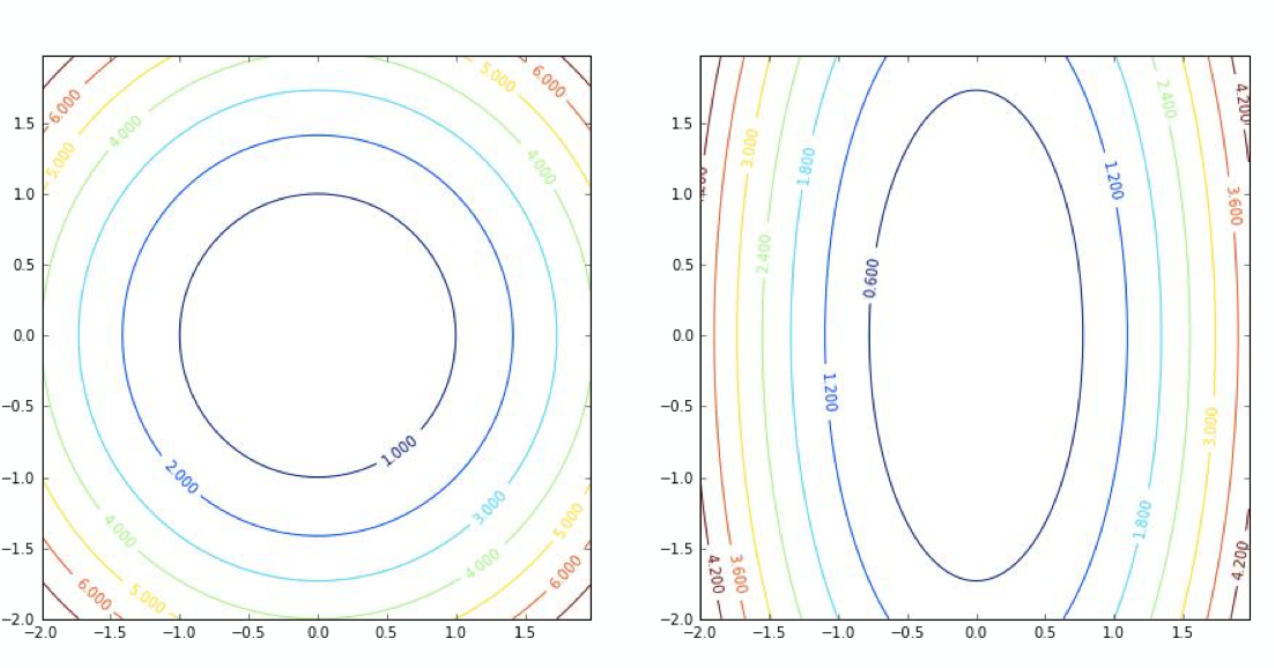
\includegraphics[width=.8\linewidth]{standartization.png}
	\end{center}
	
	\begin{center}
		Какая из ситуаций лучше для градиентного спуска? 
	\end{center}
\end{frame}


\begin{frame}{Стандартизация}
	\begin{center}
		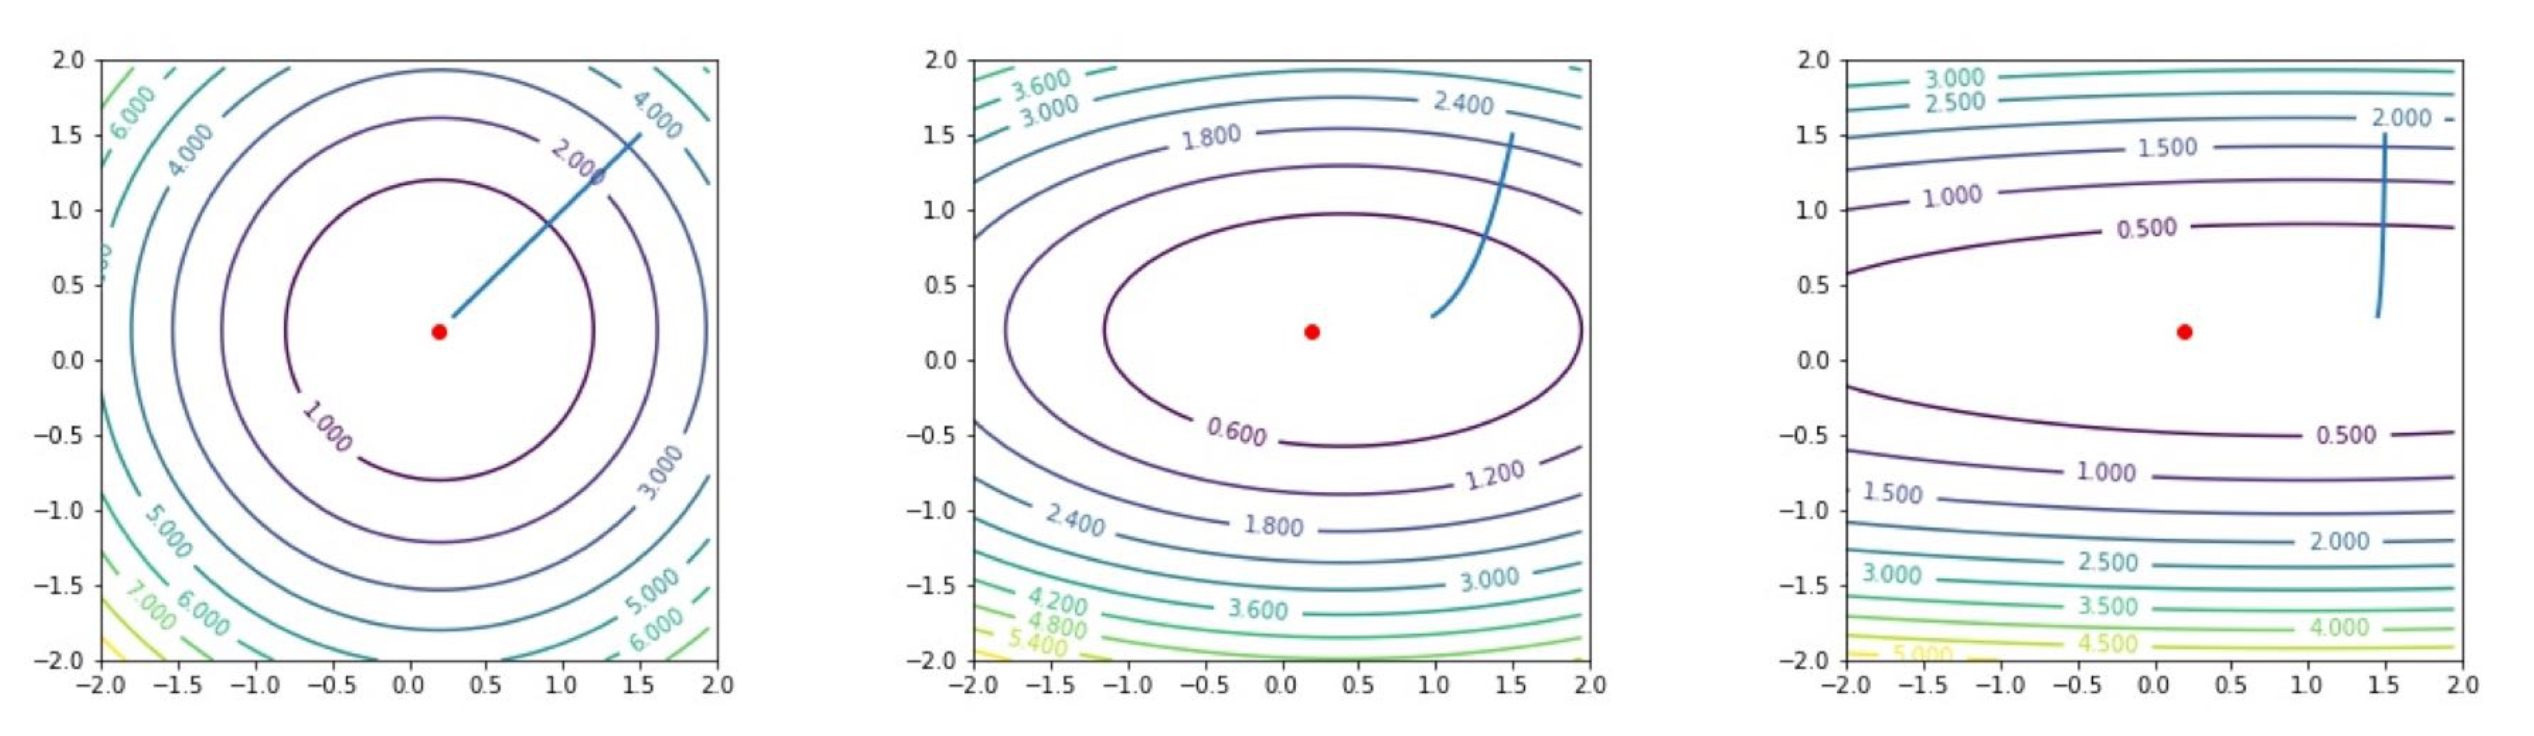
\includegraphics[width=.99\linewidth]{standartization2.png}
	\end{center}
	
	\alert{Градиентные методы быстрее сходятся, если градиенты в одном масштабе}
	
	\vfill %
	\footnotesize
	{\color{blue} \url{https://github.com/hse-aml/intro-to-dl/blob/master/week2/v2/ill-conditioned-demo.ipynb}}
\end{frame}


\begin{frame}{Стандартизация}
	Будем подавать на вход в нейросетку стандартизованные данные:
	
	\begin{equation*}
		\begin{aligned}
			&\hat{x}_{ij} = \frac{x_{ij} - \mu_j}{\sqrt{\sigma^2_j + \varepsilon}} \\
			&\mu_j = \frac{1}{n} \sum_{i=1}^n x_{ij} \\
			& \sigma^2_j =  \frac{1}{n} \sum_{i=1}^n (x_{ij} - \mu_j)^2
		\end{aligned}
	\end{equation*}
	\vfill \centering
	\alert{Это помогает градиентному спуску лучше работать}
\end{frame}


\begin{frame}{А что внутри нейросетки?}
	\begin{center}
		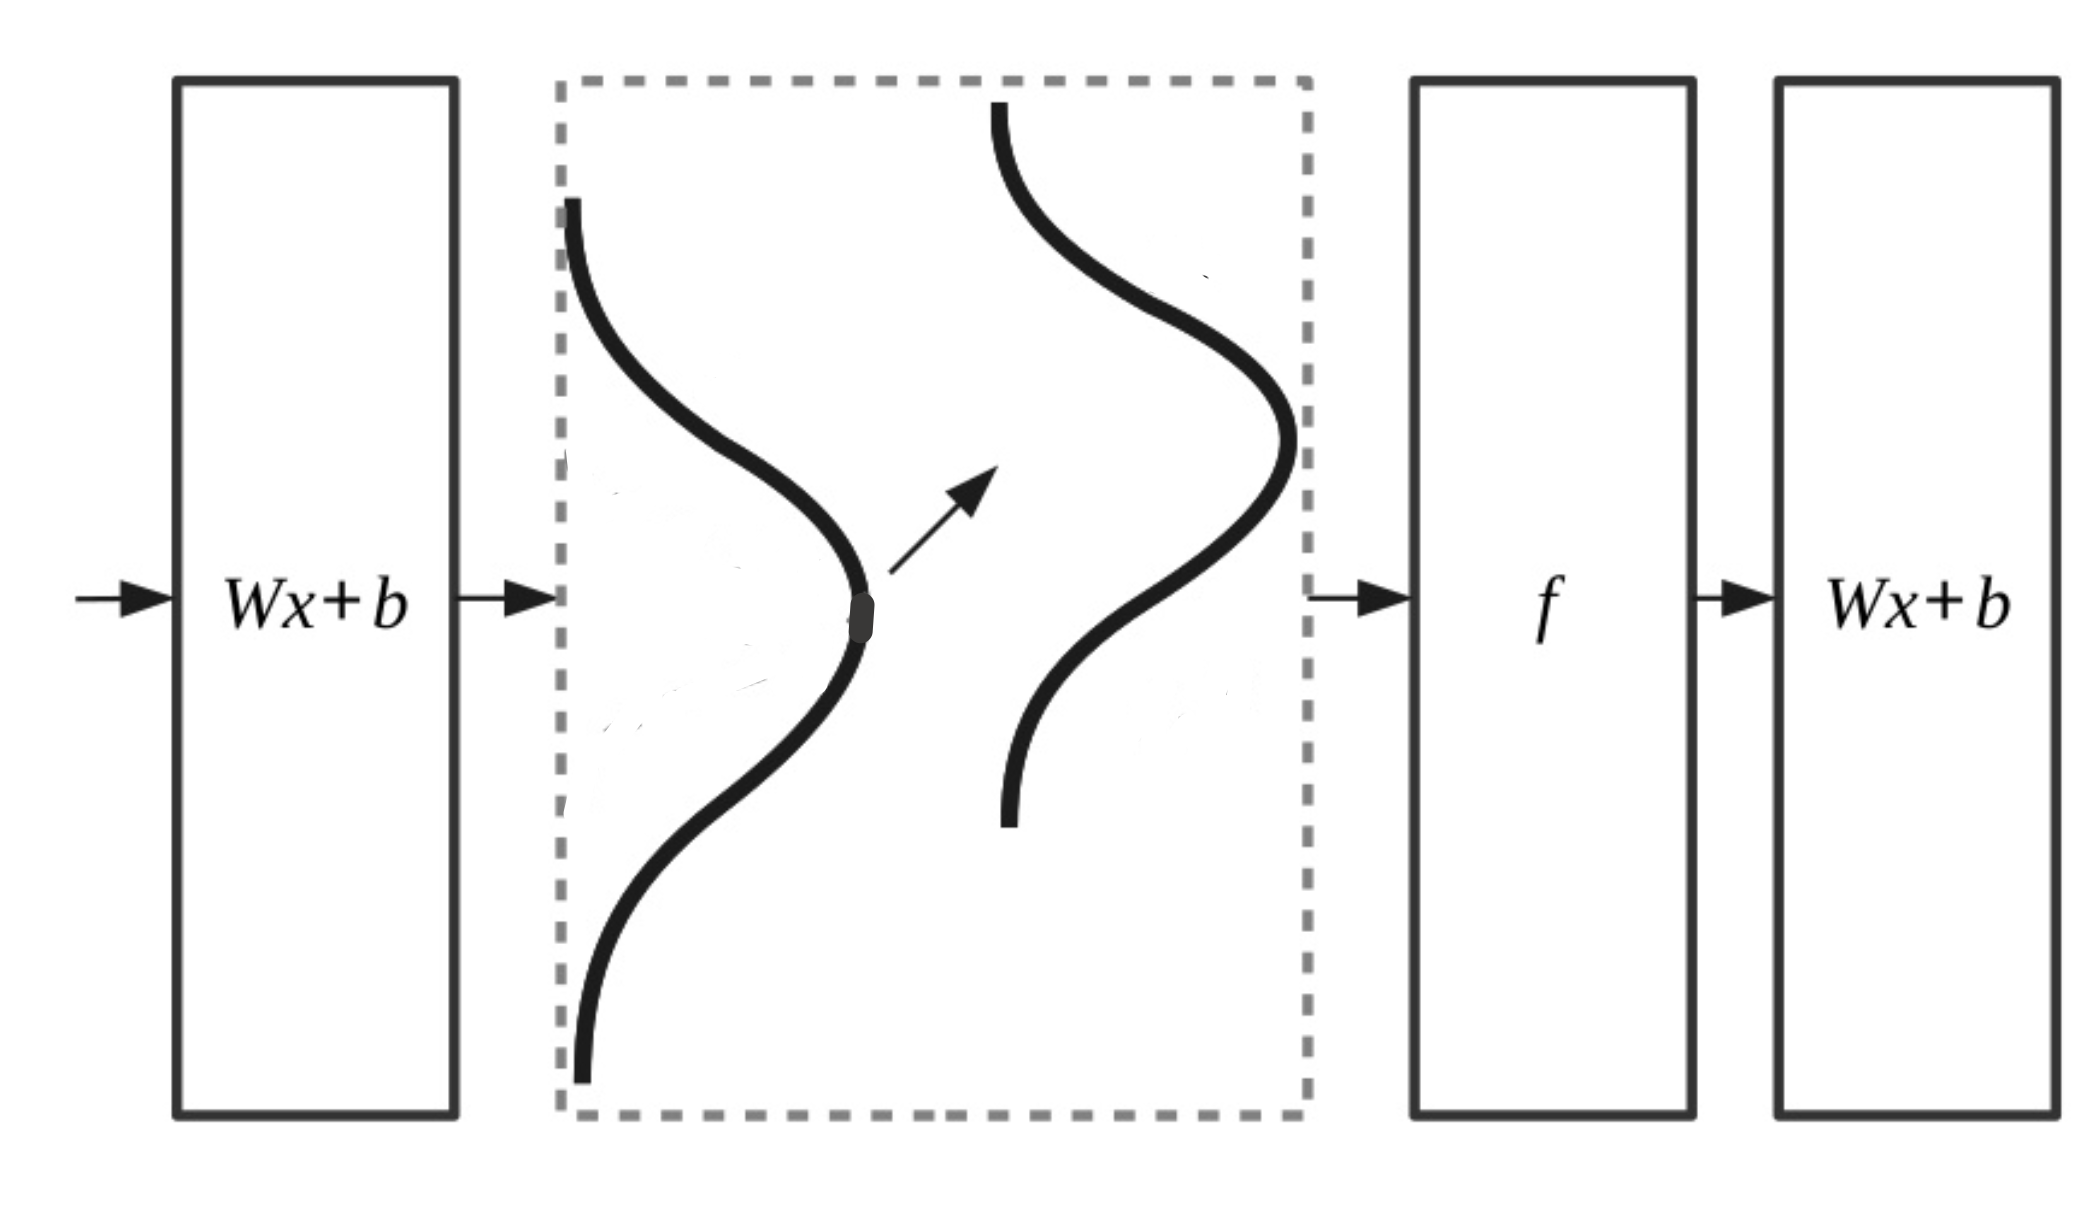
\includegraphics[width=.7\linewidth]{distributions_1.png}
	\end{center}
\end{frame}


\begin{frame}{А что внутри нейросетки?}
	\begin{center}
		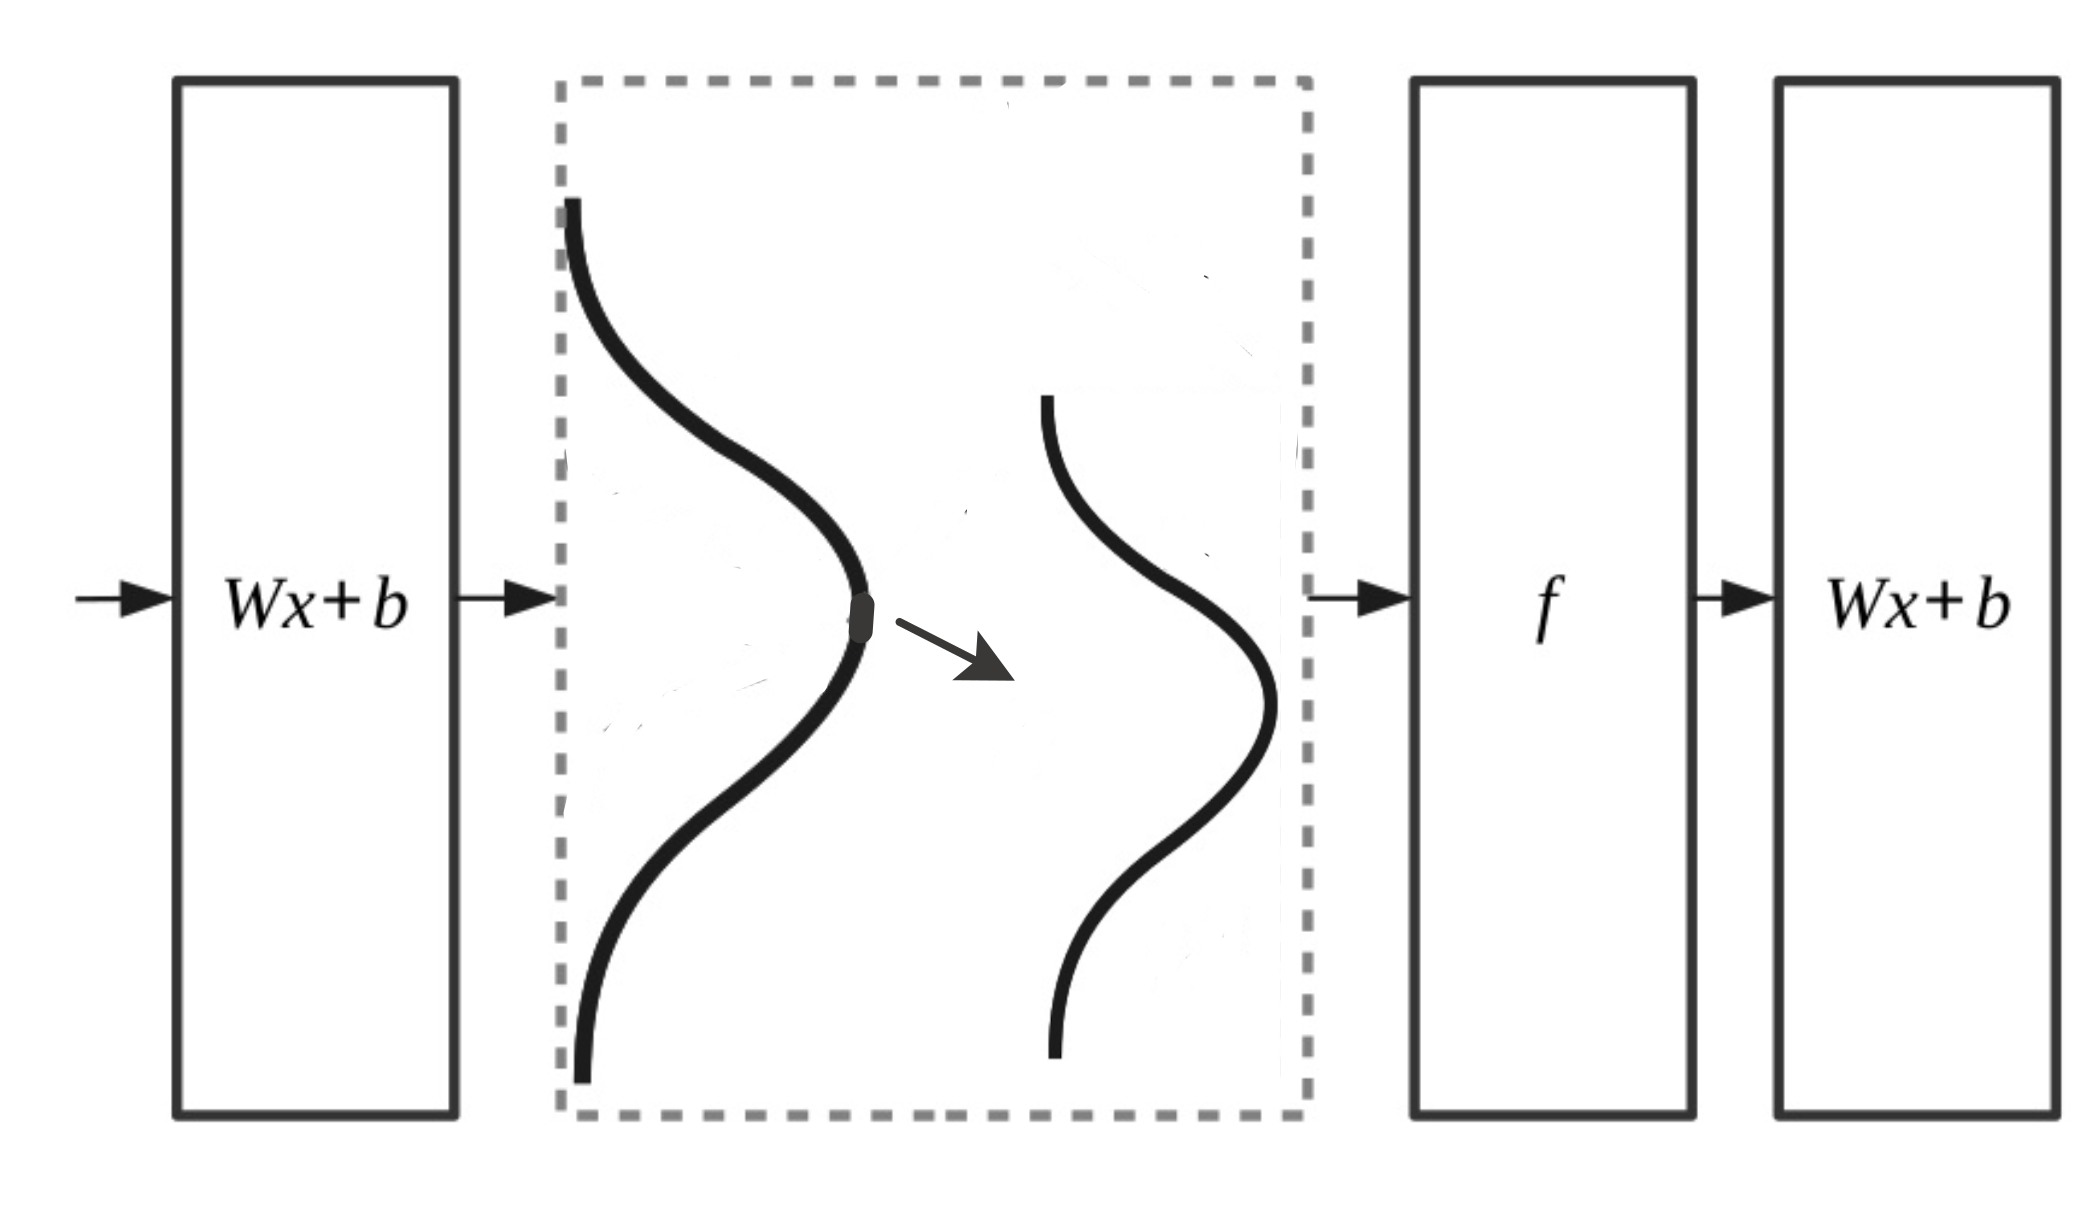
\includegraphics[width=.7\linewidth]{distributions_2.png}
	\end{center}
\end{frame}

\begin{frame}{Проблема}
	\begin{wideitemize}
		\item  Даже если мы стандартизовали вход $X$, внутри сетки может произойти несчастье и скрытый слой окажется нестандартизован 
		
		\item  Скрытые представления $h = f(XW)$  могут менять своё распределение в процессе обучения, это усложняет его  
		
		\item Давайте на каждом слое вместо $h$ использовать  $\hat{h} = \frac{h - \hat{\mu}_h}{\hat{\sigma}_h}$
		
		\item На выход будем выдавать $\beta \cdot  \hat h + \gamma$, для того, чтобы у нас было больше свободы, параметры $\beta$ и $\gamma$ учим как параметры полносвязного слоя
	\end{wideitemize}
\end{frame}


\begin{frame}{Batch Normalization (2015)}
	\begin{center}
		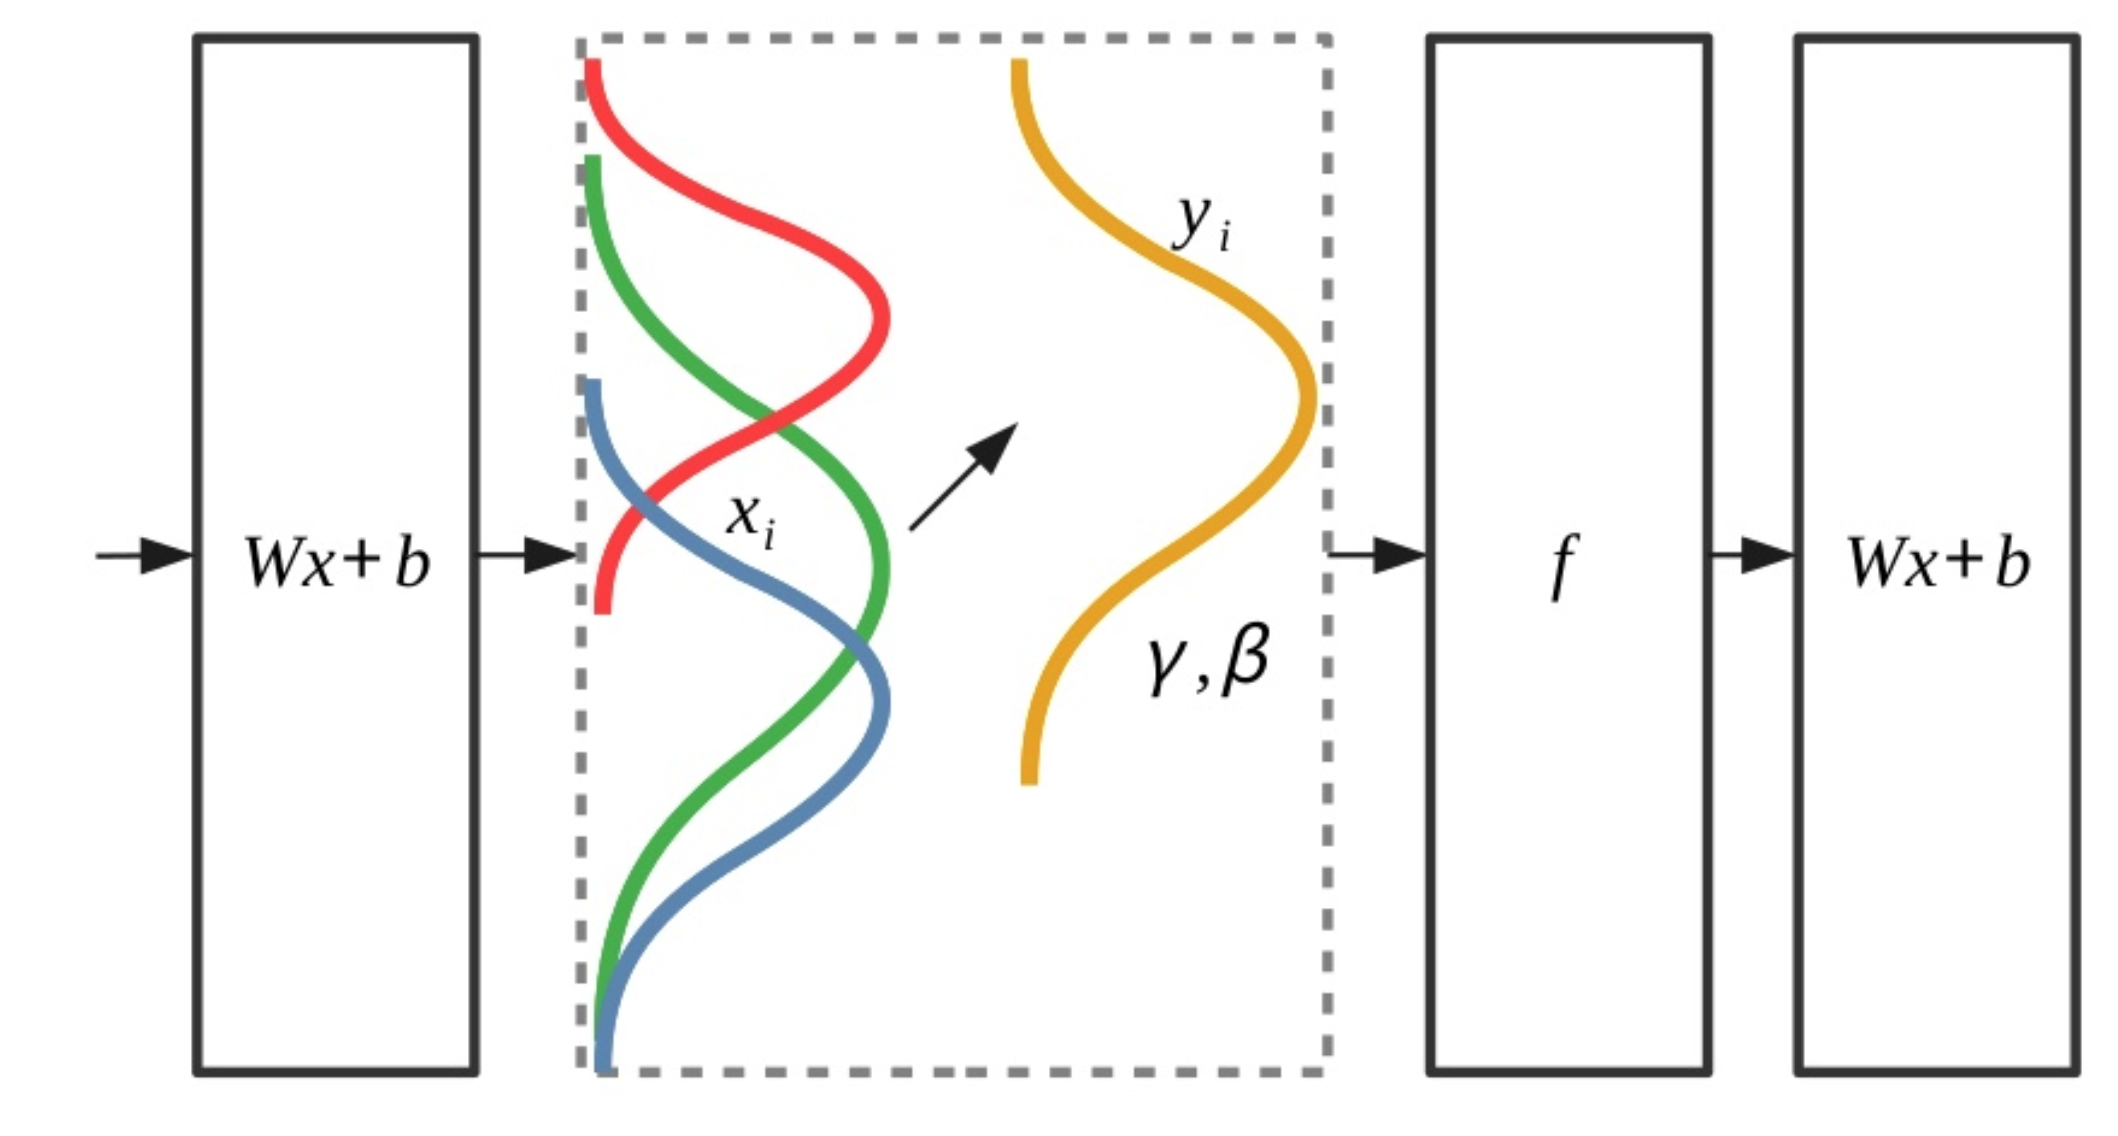
\includegraphics[width=.7\linewidth]{distributions_nice.png}
	\end{center}
\end{frame}


\begin{frame}{Forward pass}
	\begin{center}
		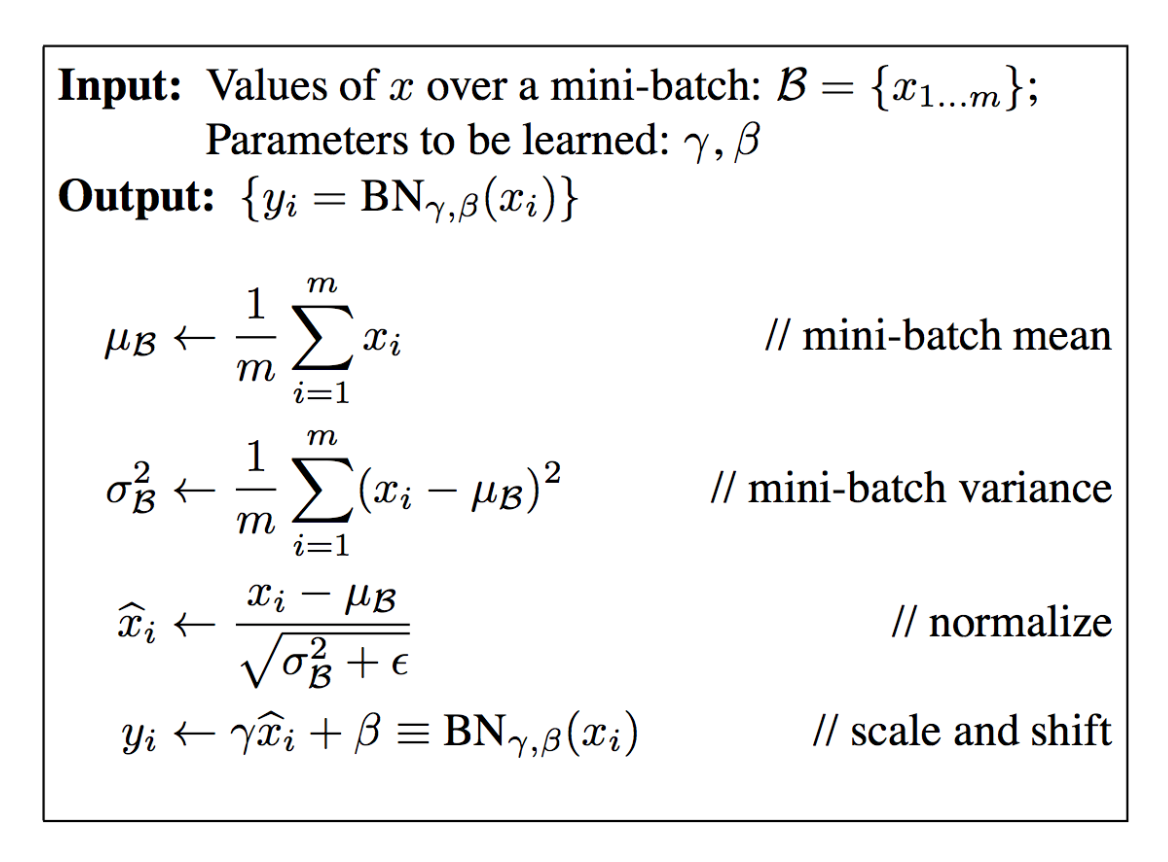
\includegraphics[width=.63\linewidth]{batch_formulas.png}
	\end{center}
	\vfill %
	\footnotesize
	{\color{blue} \url{https://arxiv.org/pdf/1502.03167.pdf}}
\end{frame}


\begin{frame}{Backward pass}
	\begin{center}
		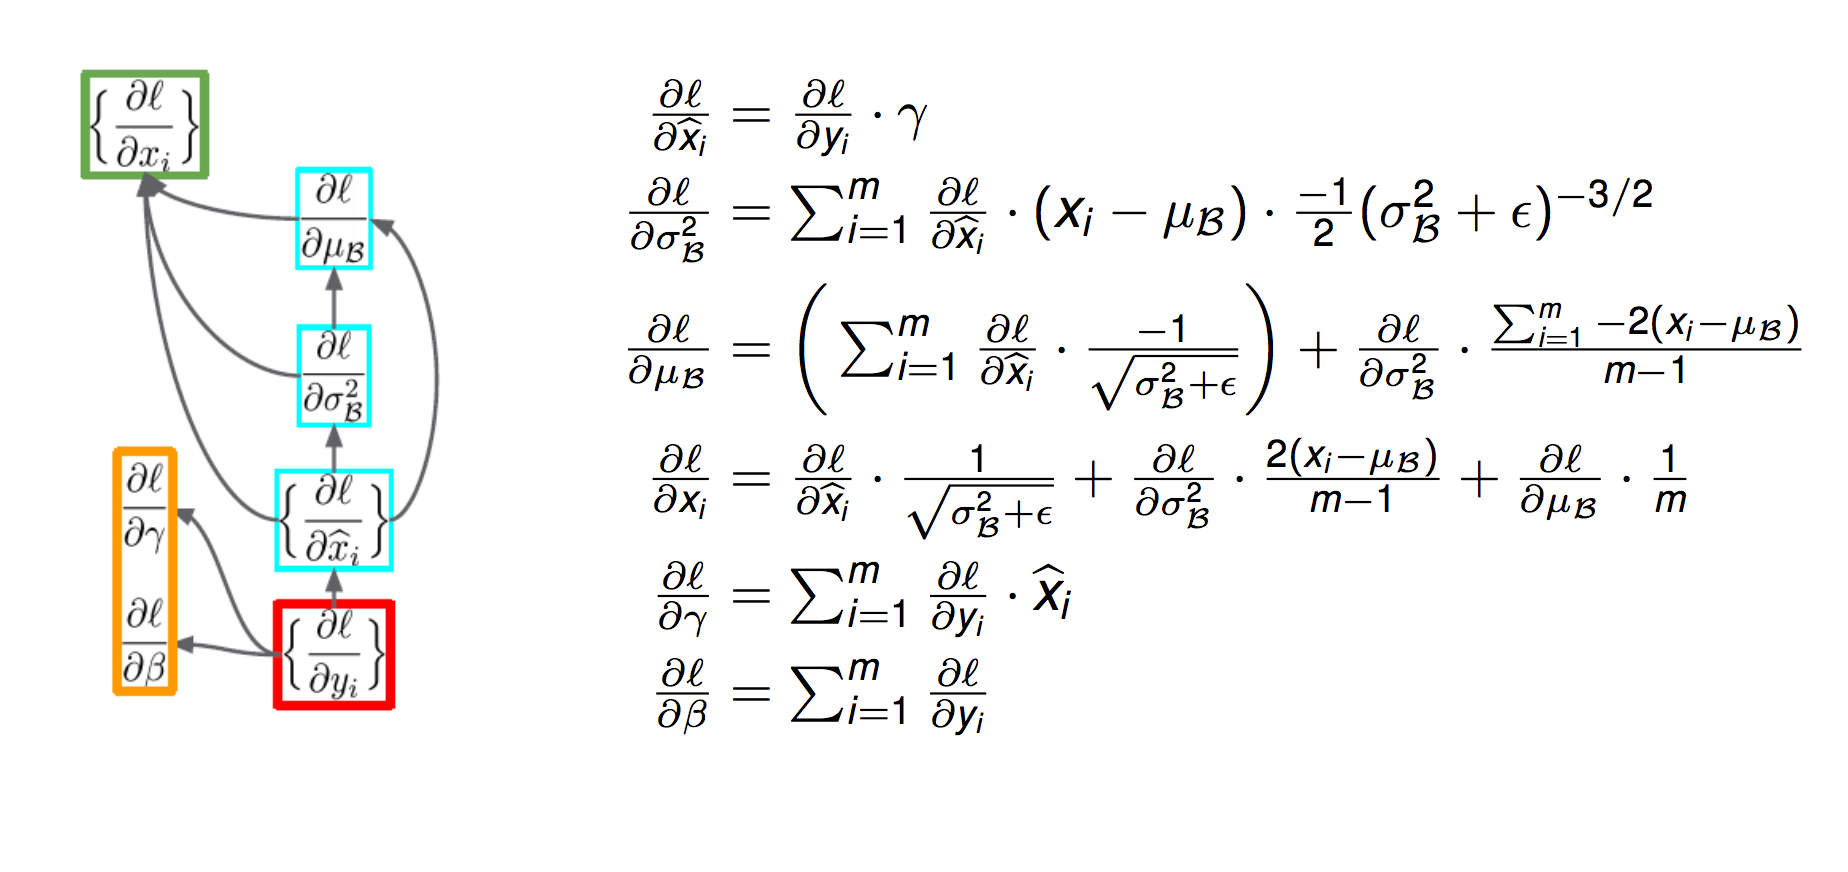
\includegraphics[width=.95\linewidth]{batch_grad.png}
	\end{center}
	\vfill %
	\footnotesize
	{\color{blue} \url{https://arxiv.org/pdf/1502.03167.pdf}}
\end{frame}


\begin{frame}{Batch Normalization (2015)}
	\begin{columns}[T] %
		\begin{column}{.3\textwidth}
			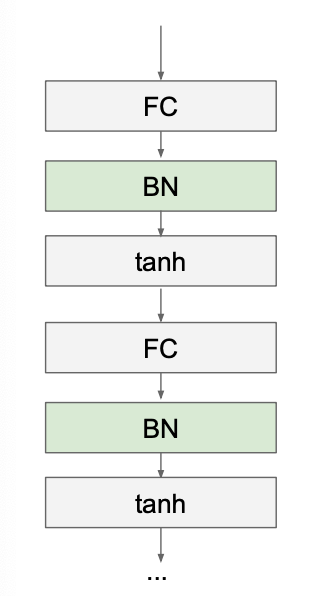
\includegraphics[width=.9\linewidth]{batch_norm_in_nn.png}
		\end{column}%
		\hfill%
		\begin{column}{.7\textwidth}
			\begin{wideitemize}
				\item  Делает обучение глубоких сетей проще
				\item Обеспечивает более высокие темпы обучения и более быструю сходимость
				\item Сети становятся более устойчивыми к инициализации
				\item Действует как регуляризатор во время обучения 
				\item \alert{Во время обучения и тестирования работает по-разному, это является источником большого числа багов и ошибок}
			\end{wideitemize}
		\end{column}%
	\end{columns}
\end{frame}


\begin{frame}{Batch norm (2015)}
	\begin{wideitemize}
		\item  Как считать $\mu_h$ и $\sigma_h$? 
		
		\item Оценить по текущему батчу! 
		
		\begin{align*} 
			\mu_h =  \alpha \cdot \bar x_{batch}  + (1 - \alpha) \cdot \mu_h \\ 
			\sigma^2_h =  \alpha \cdot \sigma^2_{batch}  + (1 - \alpha) \cdot \sigma^2_h \\ 
		\end{align*}
		
		\item Коэффициенты $\beta$ и $\gamma$ оцениваются в ходе обратного распространения ошибки, $\mu$ и $\sigma$ не обучаются
		
		\item Обучение довольно сильно ускоряется, сходимость улучшается 
	\end{wideitemize}
	\vfill %
	\footnotesize
	{\color{blue} \url{https://arxiv.org/pdf/1502.03167.pdf}}
\end{frame}


\begin{frame}{ Batch Normalization for convolutional networks}
	\begin{center}
		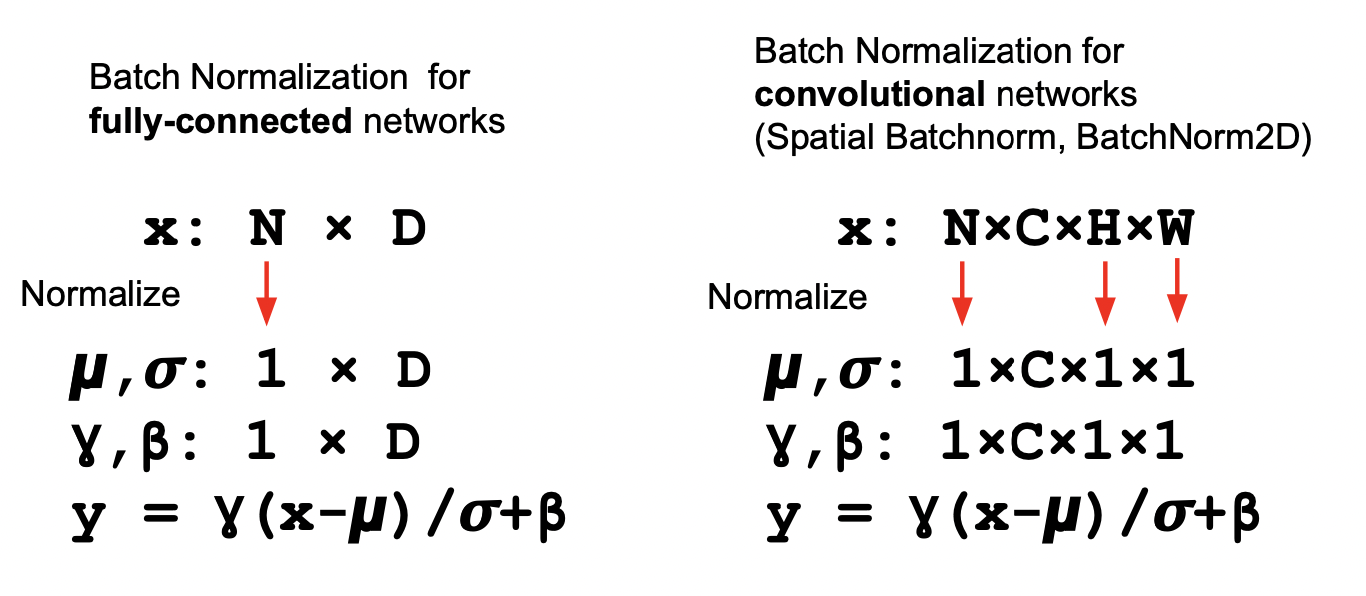
\includegraphics[width=.95\linewidth]{st_norm_1.png}
	\end{center}
	\vfill %
	\footnotesize
	Все скрины спёр у Стэнфорда, влом было набирать
\end{frame}



\begin{frame}{Layer Normalization (2016)}
	
	\begin{center}
		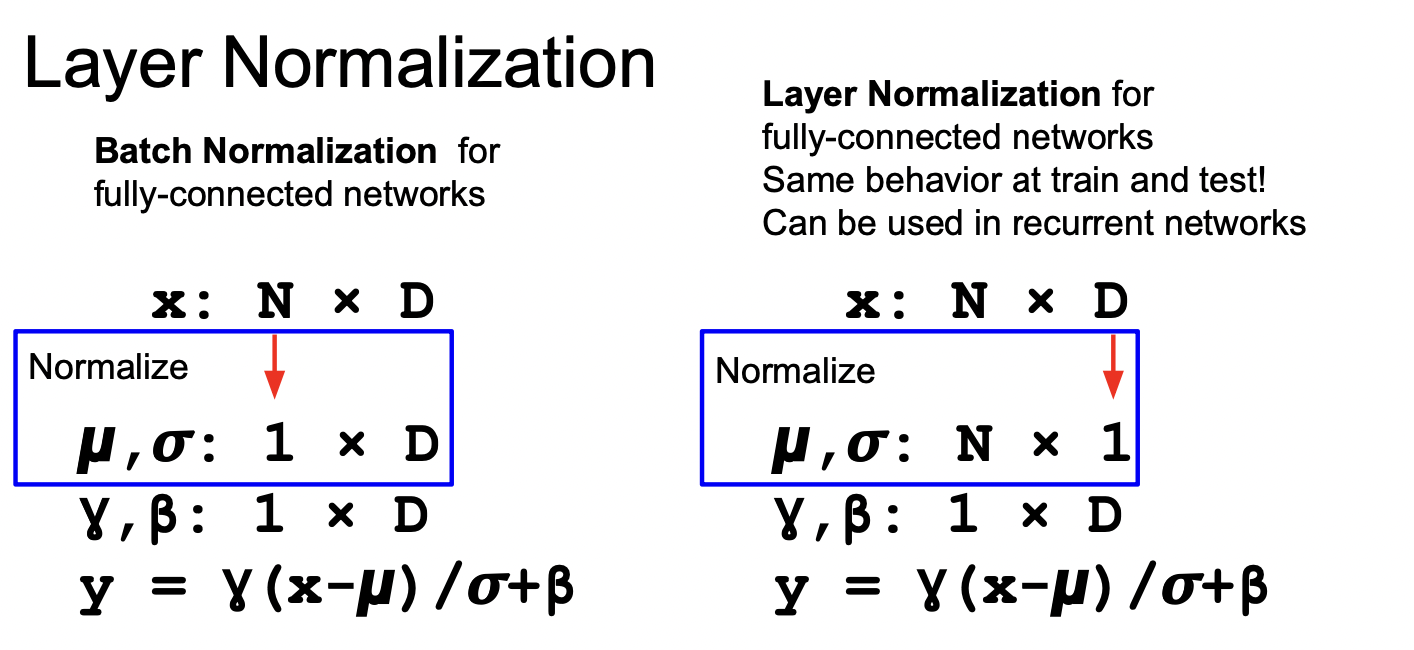
\includegraphics[width=.95\linewidth]{st_norm_2.png}
	\end{center}
	\vfill %
	\footnotesize
	{\color{blue} \url{https://arxiv.org/pdf/1607.06450.pdf}}
\end{frame}


\begin{frame}{Instance Normalization (2017)}
	\begin{center}
		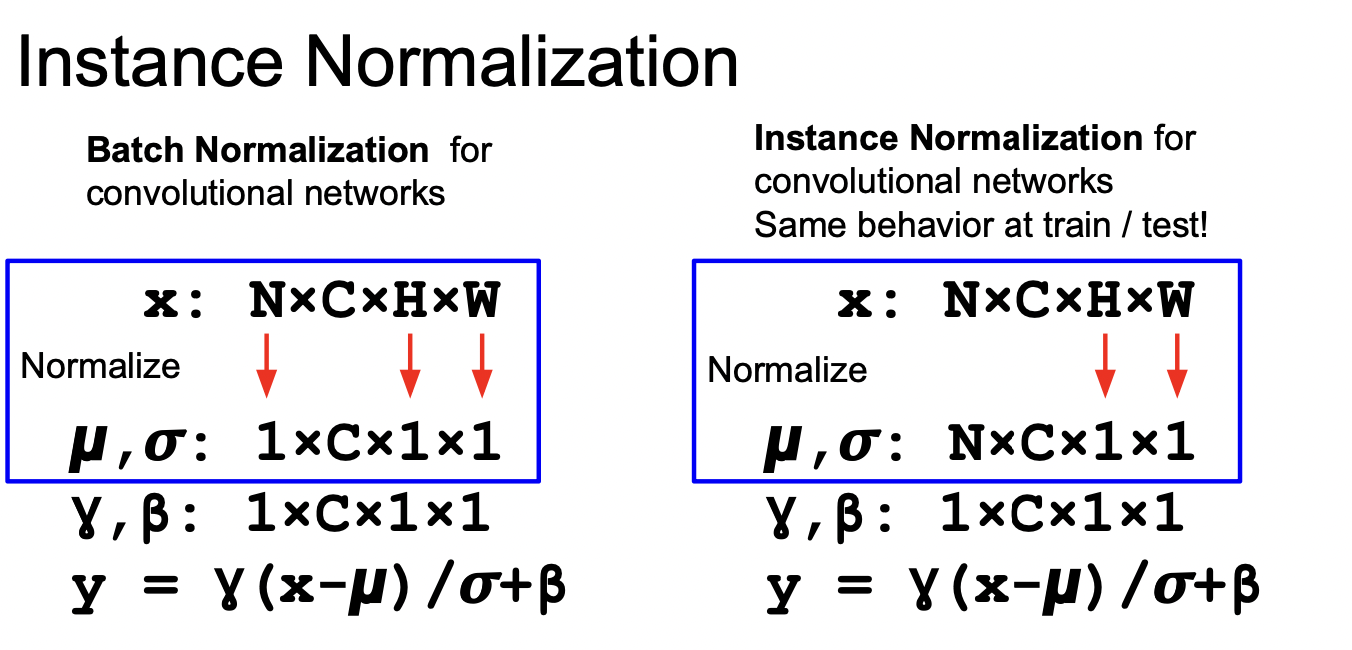
\includegraphics[width=.95\linewidth]{st_norm_3.png}
	\end{center}
\end{frame}


\begin{frame}{Сравнение слоёв для нормализации}
	\begin{center}
		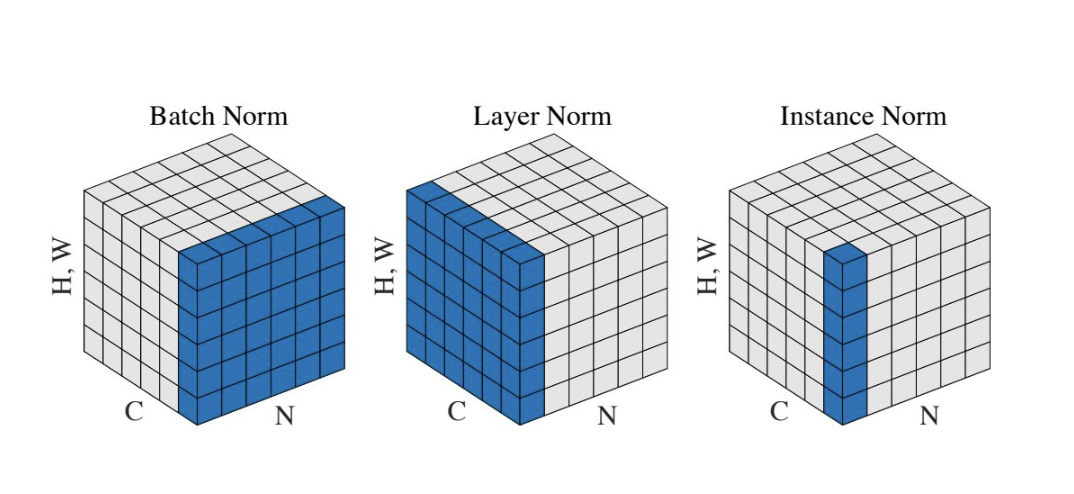
\includegraphics[width=.95\linewidth]{st_norm_4.png}
	\end{center}
\end{frame}



\begin{frame}{Почему это помогает при обучении}
	\begin{center}
		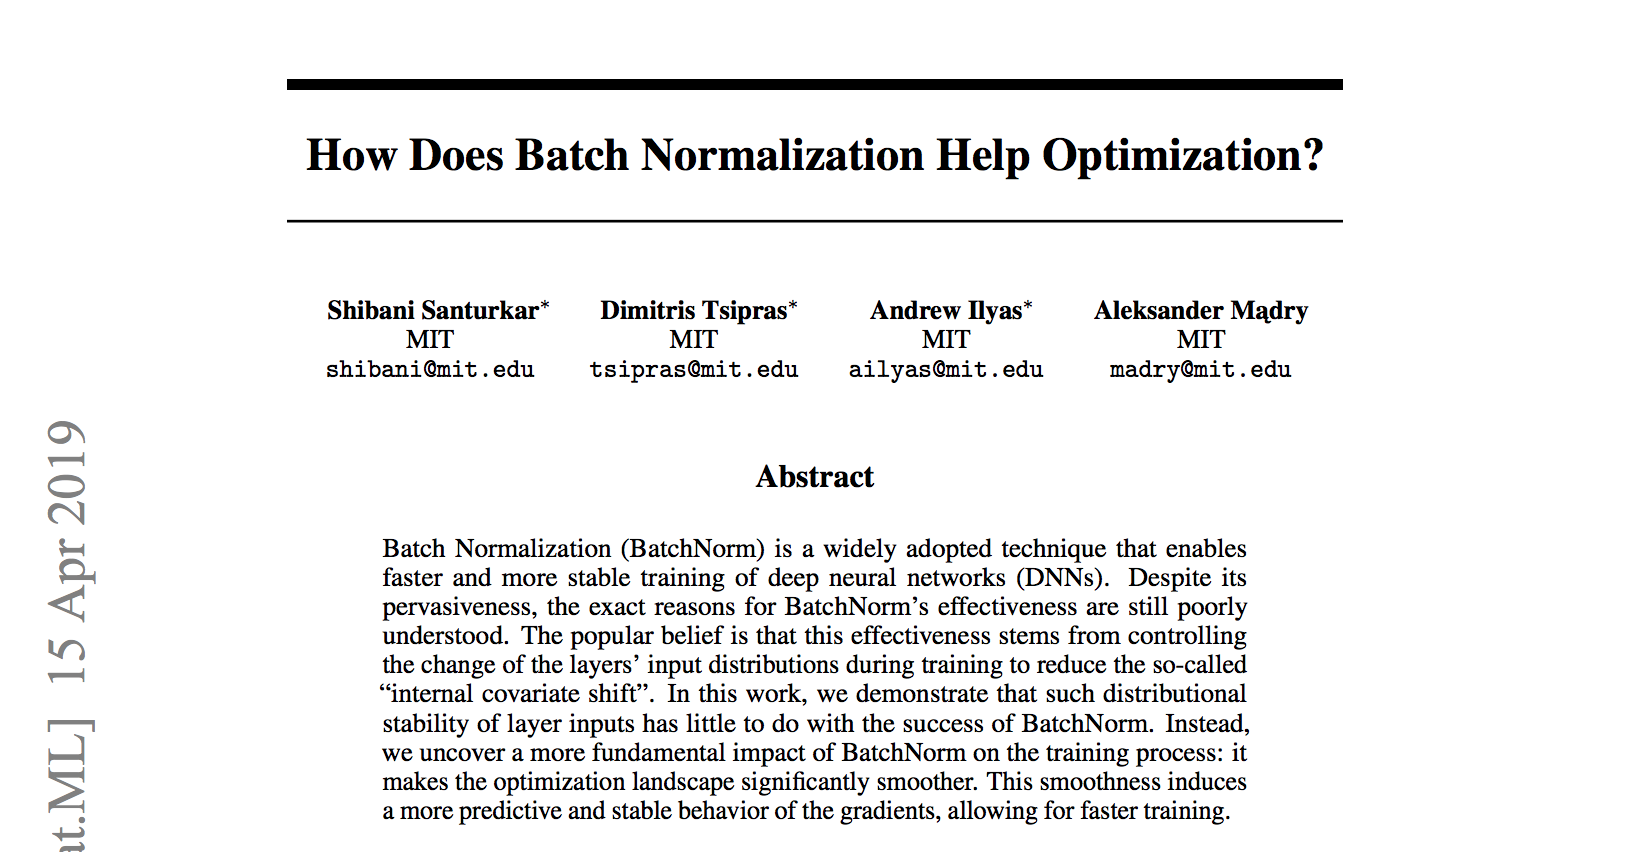
\includegraphics[width=.8\linewidth]{how_bn_help.png}
	\end{center}
	\vfill
	\footnotesize
	{\color{blue} \url{https://arxiv.org/abs/1805.11604}}
\end{frame}


\begin{frame}{Почему это помогает при обучении}
	\begin{center}
		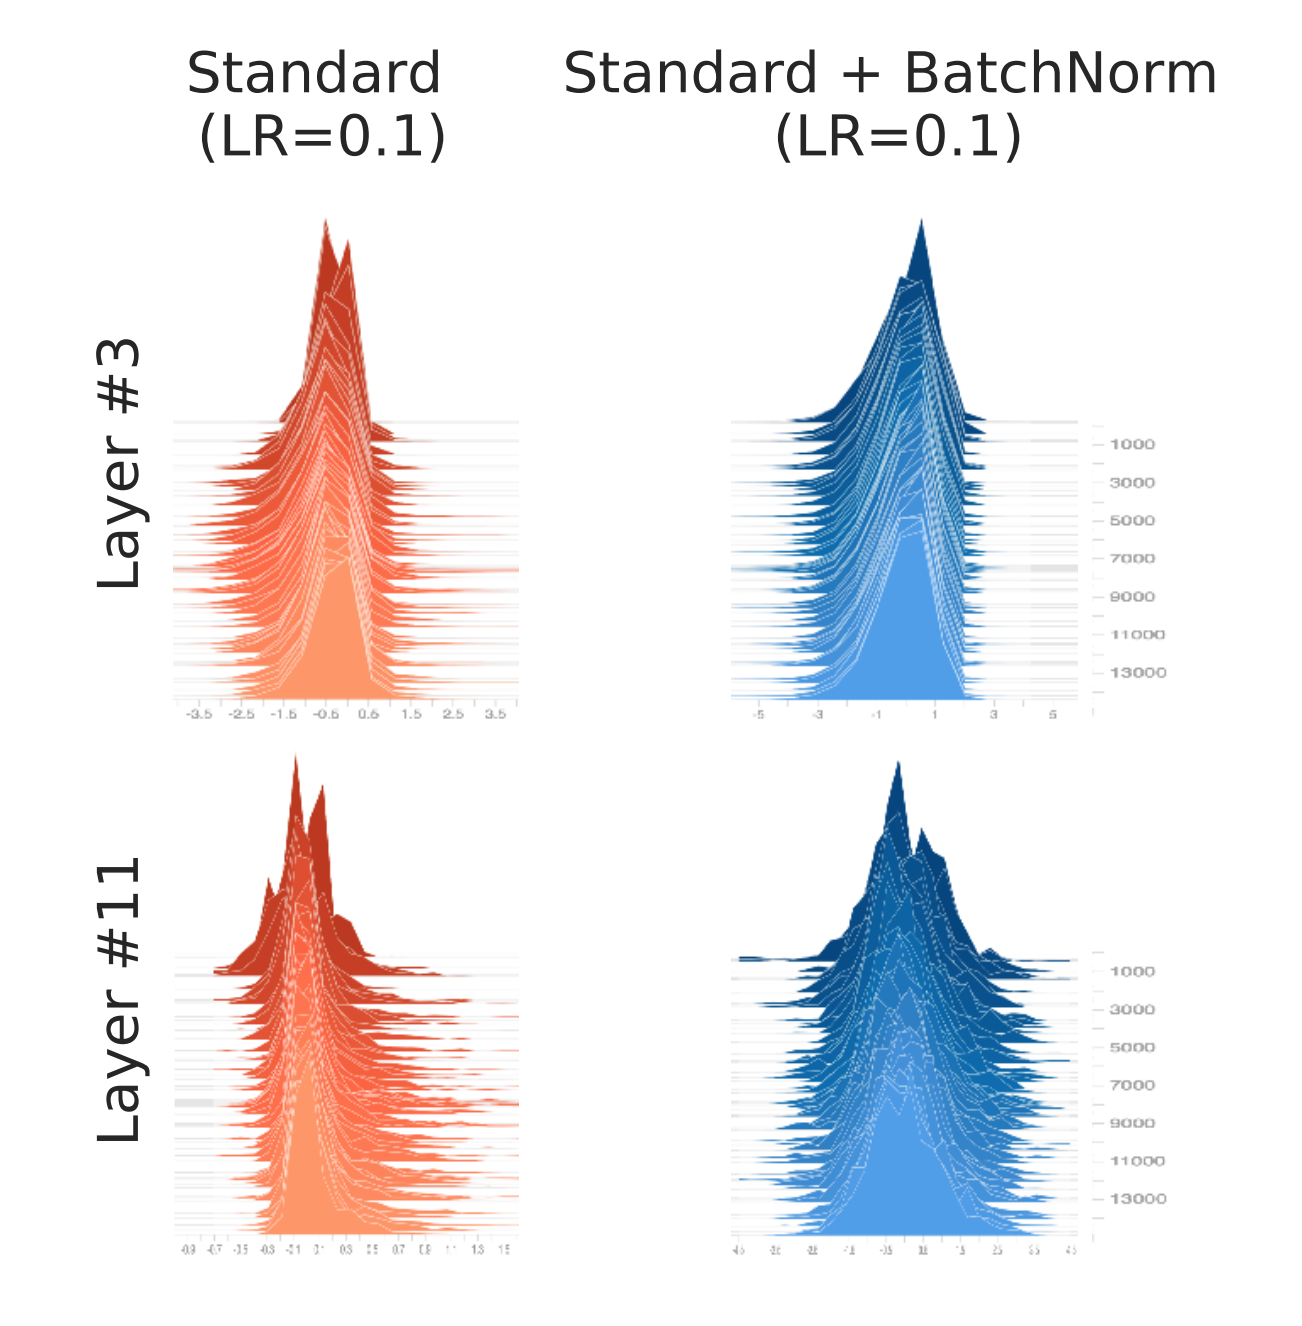
\includegraphics[width=.45\linewidth]{how_bn_help_2.png}
	\end{center}
	\vfill
	\footnotesize
	{\color{blue} \url{https://arxiv.org/abs/1805.11604}}
\end{frame}


\begin{frame}{Почему это помогает при обучении}
	\begin{center}
		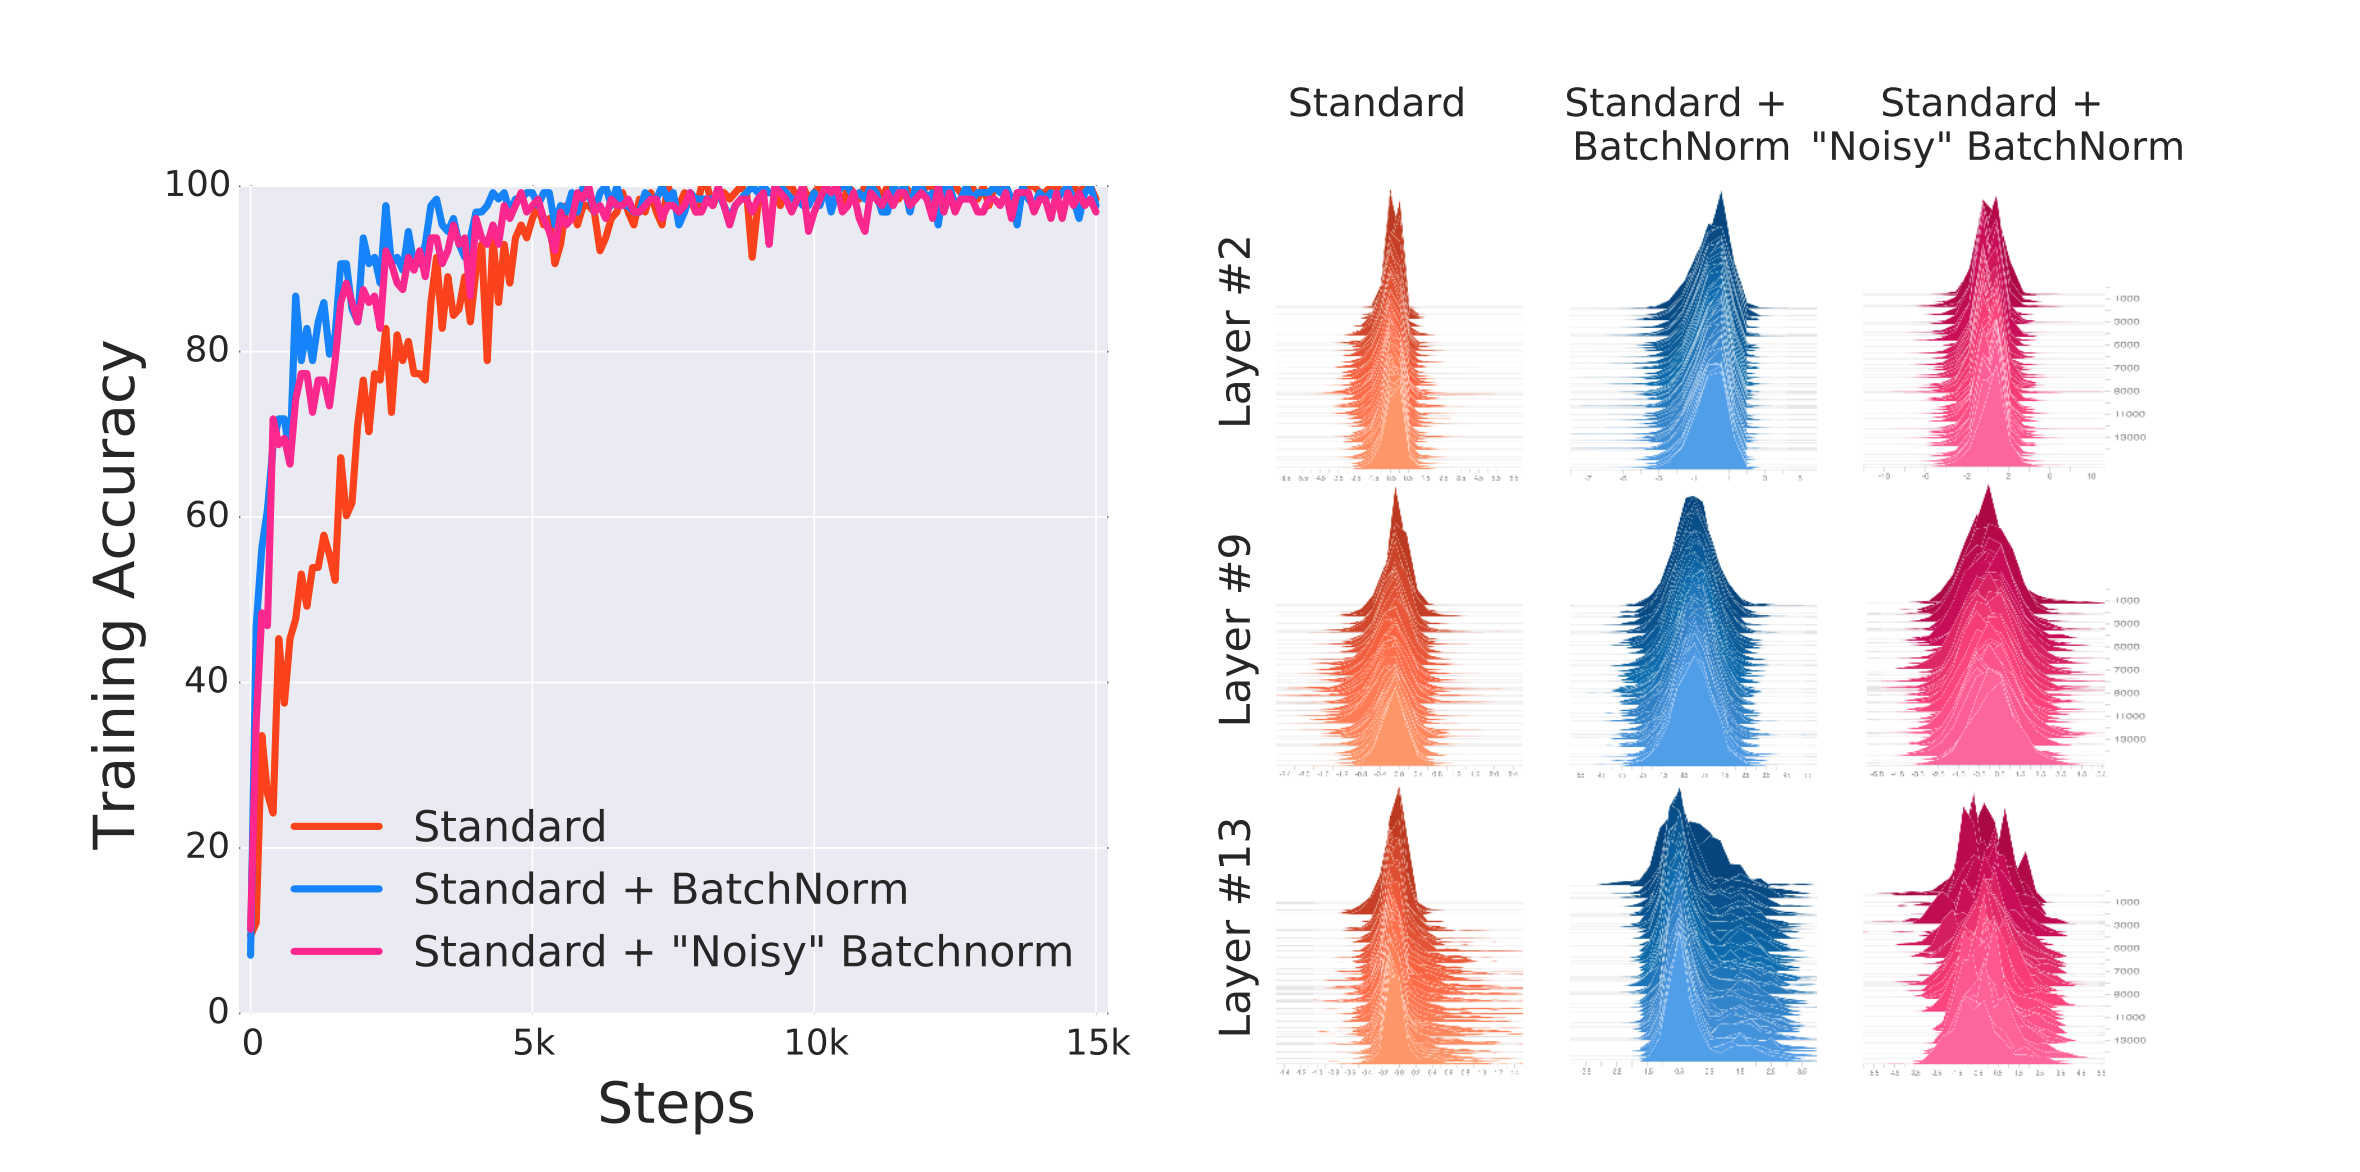
\includegraphics[width=.9\linewidth]{how_bn_help_3.png}
	\end{center}
	\vfill
	\footnotesize
	{\color{blue} \url{https://arxiv.org/abs/1805.11604}}
\end{frame}


\begin{frame}{Почему это помогает при обучении}
	\begin{center}
		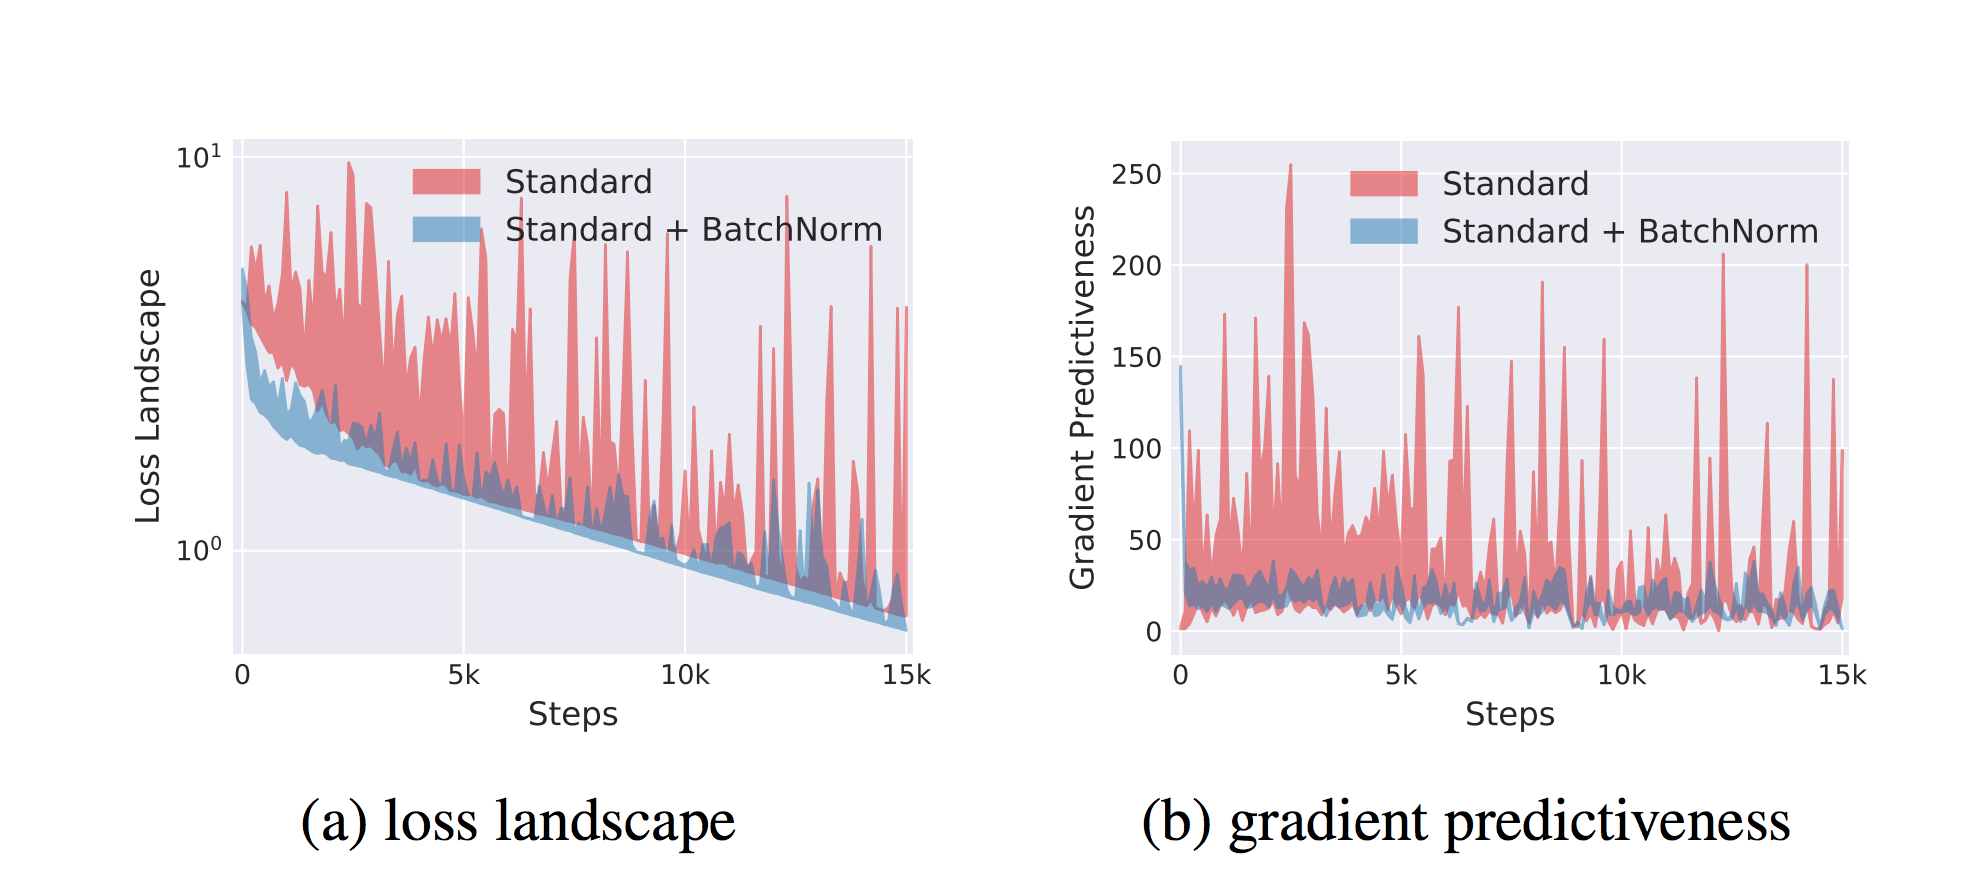
\includegraphics[width=.8\linewidth]{how_bn_help_4.png}
		
		\alert{Батчнорм сглаживает ландшафт функции потерь и из-за этого градиентный спуск идёт более гладко.}
	\end{center}
	\vfill
	\footnotesize
	{\color{blue} \url{https://arxiv.org/abs/1805.11604}}
\end{frame}


\begin{frame}{Трюки}
	\begin{wideitemize}
		\item  С батч-нормализацией нужно уменьшить силу Dropout и регуляризацию
		
		\item Батч-нормализация и Dropout могут конфликтовать 
		
		\item  Не забывайте перемешивать обучающую выборку перед каждой новой эпохой, чтобы батчи были разнообразными 
		
		\item Существует довольно много техник нормализации:  Layer Normalization, Weight Normalization, Batch Renormalization, Adaptive Instance Normalization, Group Normalization etc.	
	\end{wideitemize}
	\vspace{1 cm} %
	\footnotesize
	{\color{blue} \url{http://openaccess.thecvf.com/content_CVPR_2019/papers/Li_Understanding_the_Disharmony_Between_Dropout_and_Batch_Normalization_by_Variance_CVPR_2019_paper.pdf}}
\end{frame}





\begin{transitionframe}
	\begin{center}
		\Huge  Инициализация весов
	\end{center}
	\centering 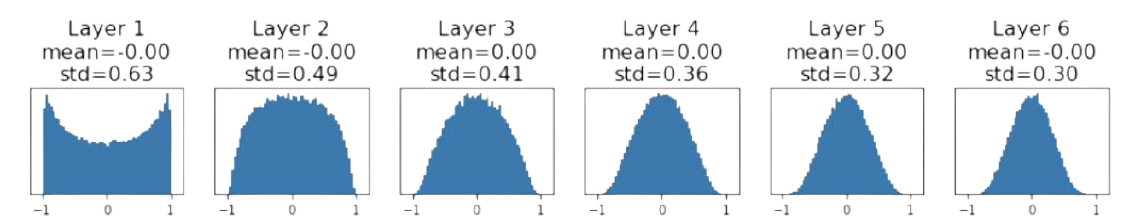
\includegraphics[width=.8\linewidth]{glorot_init_hist-removebg-preview.png}
\end{transitionframe}


\begin{frame}{Инициализация весов}
	\begin{center}
		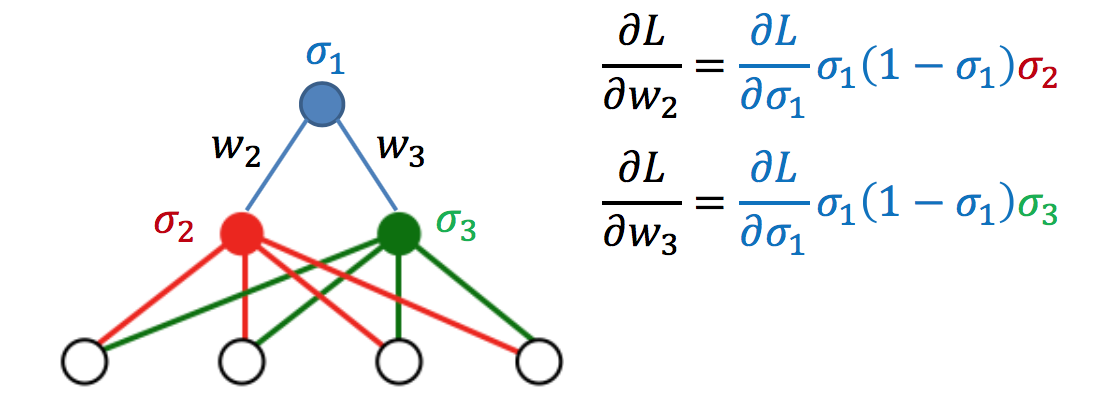
\includegraphics[width=.6\linewidth]{init1.png}
	\end{center}
	\begin{wideitemize}
		\item  Что будет, если инициализировать веса нулями?  \pause 
		\item  ${\color{red} \sigma_2 }$ и ${\color{green} \sigma_3 }$  будут обновляться одинаково
	\end{wideitemize}
\end{frame}


\begin{frame}{Инициализация весов}
	\begin{center}
		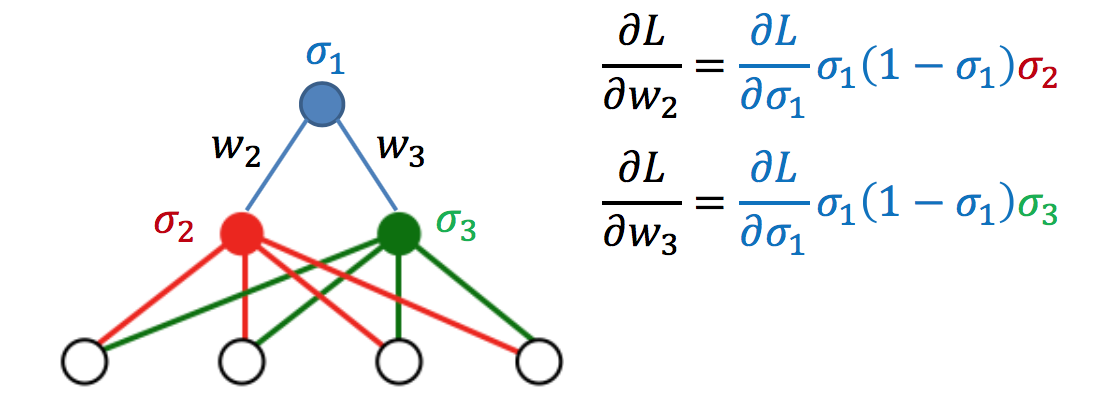
\includegraphics[width=.6\linewidth]{init1.png}
	\end{center}
	\begin{wideitemize}
		\item  Хочется уничтожить симметрию
		\item  Можно инициализировать маленькими рандомными числами из какого-то распределения (нормальное, равномерное)
		\item {\color{red}  Это будет плохо работать для глубоких сетей} 
	\end{wideitemize}
\end{frame}


% Тут мне пиздец было влом настраивать minted и я упоролся
\begin{frame}{Инициализация весов}
\begin{columns}
	\begin{column}{.45\textwidth}
		\only<1-2>{		
		\begin{wideitemize} 
		 \item Прямой проход через 6 слоёв нейросети
		 \item \alert{Что произойдёт с активацией к последнему слою?}
		 \only<2>{\item Активация постепенно стягивается к нулю }
		\end{wideitemize}}
	\only<3-4>{
	\begin{wideitemize} 
			\item Активация постепенно стягивается к нулю
			\item \alert{А что будет происходить с градиентами?}
			\only<4>{\item Все будут нулевыми :(  }
	\end{wideitemize}}
	\end{column}
	\begin{column}{.55\textwidth}
		dims = [{\color{green} 4096}] *  {\color{green} 7} \\
		hs = [ ] \\
		x = np.random.randn(  {\color{green} 16}, dims[  {\color{green} 0} ]) \\
		{\color{green} for} Din, Dout {\color{green} in zip}(dims[:  {\color{green} -1}], dims[ {\color{green} 1}:]): \\  
		\mbox{ } \hspace{5mm} W =  {\color{green} 0.01} * np.random.randn(Din, Dout) \\
		\mbox{ } \hspace{5mm} x = np.tanh(x.dot(W)) \\
		\mbox{ } \hspace{5mm} hs.append(x)
	\end{column}
\end{columns}
\hfill \only<2->{
\begin{center}
	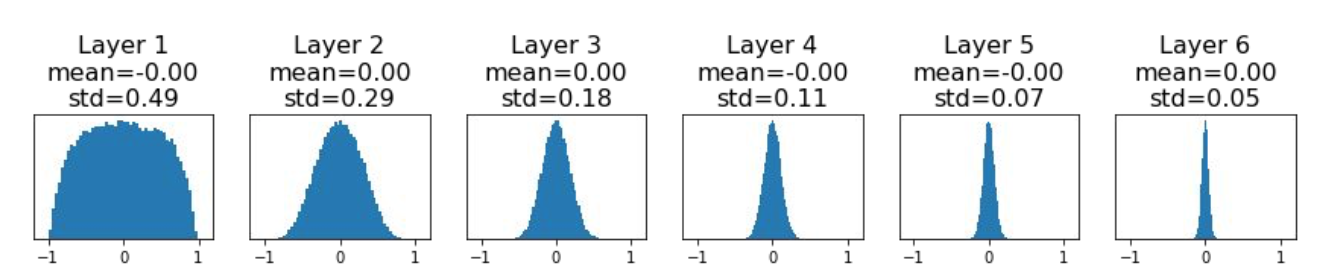
\includegraphics[width=.99\linewidth]{init_tanh_activation.png}
\end{center}}
\end{frame}


\begin{frame}{Инициализация весов}
\begin{columns}
	\begin{column}{.45\textwidth}
		\only<1-2>{		
			\begin{wideitemize} 
				\only<1>{\item Увеличим стандартное отклонение в инициализации с $0.01$ до $0.05$
				\item \alert{Что произойдёт с активацией к последнему слою?}}
				\only<2>{\item Постепенно происходит насыщение, \alert{градиенты опять занулятся} }
		\end{wideitemize}}
	\end{column}
	\begin{column}{.55\textwidth}
		dims = [{\color{green} 4096}] *  {\color{green} 7} \\
		hs = [ ] \\
		x = np.random.randn(  {\color{green} 16}, dims[  {\color{green} 0} ]) \\
		{\color{green} for} Din, Dout {\color{green} in zip}(dims[:  {\color{green} -1}], dims[ {\color{green} 1}:]): \\  
		\mbox{ } \hspace{5mm} W =  {\color{red} \textbf {0.05} } * np.random.randn(Din, Dout) \\
		\mbox{ } \hspace{5mm} x = np.tanh(x.dot(W)) \\
		\mbox{ } \hspace{5mm} hs.append(x)
	\end{column}
\end{columns}
\hfill \only<2->{
	\begin{center}
		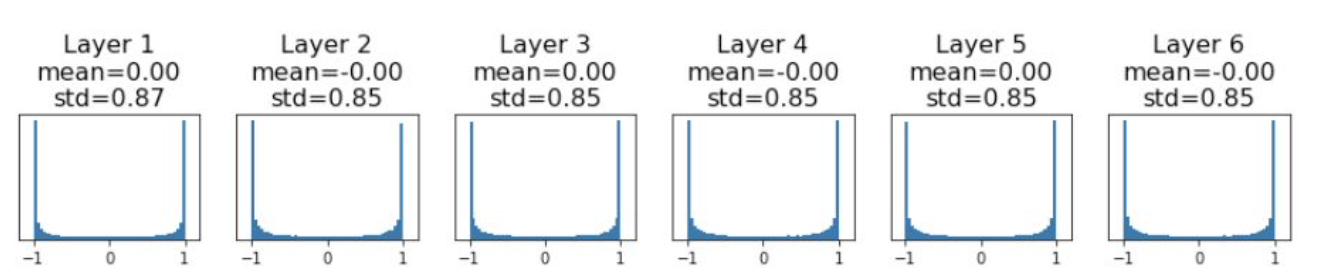
\includegraphics[width=.99\linewidth]{bad_init_tanh.png}
\end{center}}
\end{frame}


\begin{frame}{Инициализация весов}
\begin{columns}
	\begin{column}{.3\textwidth}	
			\begin{wideitemize} 
				\item Распределение активаций не меняется,  \alert{с градиентами всё хорошо}
		\end{wideitemize}
	\end{column}
	\begin{column}{.7\textwidth}
		dims = [{\color{green} 4096}] *  {\color{green} 7} \\
		hs = [ ] \\
		x = np.random.randn(  {\color{green} 16}, dims[  {\color{green} 0} ]) \\
		{\color{green} for} Din, Dout {\color{green} in zip}(dims[:  {\color{green} -1}], dims[ {\color{green} 1}:]): \\  
		\mbox{ } \hspace{5mm} W =  {\color{red} \textbf {1/np.sqrt(Din)} } * np.random.randn(Din, Dout) \\
		\mbox{ } \hspace{5mm} x = np.tanh(x.dot(W)) \\
		\mbox{ } \hspace{5mm} hs.append(x)
	\end{column}
\end{columns}
	\begin{center}
		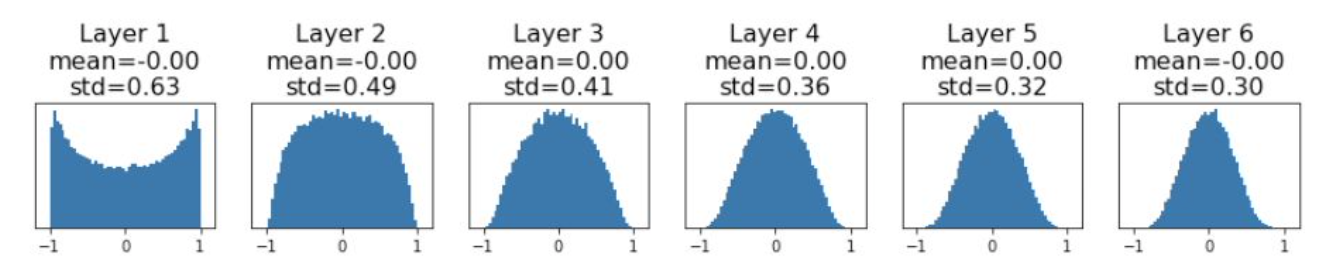
\includegraphics[width=.99\linewidth]{glorot_init_hist.png}
\end{center}
\end{frame}


\begin{frame}{Инициализация весов}
	\begin{wideitemize}
		\item  Посмотрим на выход нейрона перед активацией:
	\begin{equation*}
		\begin{aligned} 
			h_i =  \sum_{i=1}^{n_{in}} w_i x_i 
		\end{aligned}
	\end{equation*}
		\item  Дисперсия $h_i$ выражается через дисперсии $x$ и $w$ 
		\item Будем считать, что веса $w_1, \ldots, w_k \sim iid$,  наблюдения $x_1, \ldots, x_n \sim iid$, а ещё $x_i$ и $w_i$ независимы между собой
	\end{wideitemize}
\end{frame}


\begin{frame}{Инициализация весов (симметричная активация)}
\begin{multline*} 	
\Var(h_i) = \Var(\sum_{i=1}^{n_{in}} w_i x_i) =  \sum_{i=1}^{n_{in}} \Var(w_i x_i) = \\ 
= \sum_{i=1}^{n_{in}} [\E(x_i)]^2 \cdot \Var(w_i) + [\E(w_i)]^2 \cdot \Var(x_i)  + \Var(x_i) \cdot \Var(w_i)] = \only<3->{\\  =  \sum_{i=1}^{n_{in}}  \Var(x_i) \cdot \Var(w_i)  } \only<4>{ =  \Var(x)  \color{green} \cdot [n_{in} \cdot \Var(w)]} \only<5->{ =  \Var(x)  \color{green} \cdot \underbrace{[n_{in} \cdot \Var(w)]}_{= 1}}
\end{multline*}
\only<2-4>{

\begin{wideitemize}
\only<2>{ \item  Если функция активации симметричная, тогда $E(x_i) = 0$. Будем инициализировать веса с нулевым средним, тогда $E(w_i) = 0$.}

\only<3>{ 
\item  Предполагаем, что $x_i$ инициализируются из одного распределения, $w_i$ сами инициализируем из одного распределения.}

\only<4>{ 
\item  Хотим, чтобы зелёная штука была равна единице, тогда у потока будет всегда постоянная дисперсия, совпадающая с $\Var(x)$.}
\end{wideitemize}}

\only<1>{
\vspace{3cm}
\footnotesize
{\color{blue}  \url{https://en.wikipedia.org/wiki/Variance\#Product\_of\_independent\_variables}}}
\end{frame}


\begin{frame}{Плохая инициализация весов}
	Пусть
	
	$$ w_i \sim U \left[ - \frac{1}{\sqrt{n_{in}}};  \frac{1}{\sqrt{n_{in}}}  \right],$$
	
	тогда 
	
	$$
	\Var(w_i) = \frac{1}{12} \cdot \left( \frac{1}{\sqrt{n_{in}}} + \frac{1}{\sqrt{n_{in}}} \right)^2 = \frac{1}{3 n_{in}} \Rightarrow Var(h_i) = \frac{1}{3} 
	$$
	
	\alert{Получаем затухание!}
\end{frame}


\begin{frame}{Инициализация Ксавье/Глорота (2010)}
	Пусть
	
	$$ w_i \sim U \left[ - \frac{\sqrt{3}}{\sqrt{n_{in}}};  \frac{\sqrt{3}}{\sqrt{n_{in}}}  \right],$$
	
	тогда 
	
	$$
	\Var(w_i) = \frac{1}{12} \cdot \left( \frac{\sqrt{3}}{\sqrt{n_{in}}} + \frac{\sqrt{3}}{\sqrt{n_{in}}} \right)^2 = \frac{1}{n_{in}} \Rightarrow Var(h_i) = 1 \pause 
	$$
	
	\vfill 
	При forward pass на вход идёт $n_{in}$ наблюдений, при backward pass на вход идёт $n_{out}$ градиентов $\Rightarrow$   \alert{канал с дисперсией может быть непостоянным, если число весов от слоя к слою сильно колеблется}
\end{frame}


\begin{frame}{Инициализация Ксавье/Глорота (2010)}
	\begin{wideitemize}
		\item Для неодинаковых размеров слоёв невозможно удовлетворить обоим условиям, поэтому обычно усредняют и пытаются инициализировать веса с дисперсией $$\frac{2}{n_{in} + n_{out}}$$
		
		\item Такая инициализация называется \alert{инициализацией Ксавие (или Глорота)}
	
		$$ w_i \sim U \left[ - \frac{\sqrt{6}}{\sqrt{n_{out} + n_{in}}};  \frac{\sqrt{6}}{\sqrt{n_{out} + n_{in}}}  \right],$$
		
	\end{wideitemize}
	\vfill %
	\footnotesize
	{\color{blue} \url{http://proceedings.mlr.press/v9/glorot10a/glorot10a.pdf}}
\end{frame}


\begin{frame}{А что с ReLU?}
	\begin{columns}
	\begin{column}{.3\textwidth}	
		Инициализация Ксавье предполагает симметричную функцию активации
	\end{column}
	\begin{column}{.7\textwidth}
		dims = [{\color{green} 4096}] *  {\color{green} 7} \\
		hs = [ ] \\
		x = np.random.randn(  {\color{green} 16}, dims[  {\color{green} 0} ]) \\
		{\color{green} for} Din, Dout {\color{green} in zip}(dims[:  {\color{green} -1}], dims[ {\color{green} 1}:]): \\  
		\mbox{ } \hspace{5mm} W =  1/np.sqrt(Din) * np.random.randn(Din, Dout) \\
		\mbox{ } \hspace{5mm} {\color{red} \textbf {x = np.max(0, x.dot(W))} } \\
		\mbox{ } \hspace{5mm} hs.append(x)
	\end{column}
\end{columns}
\begin{center}
	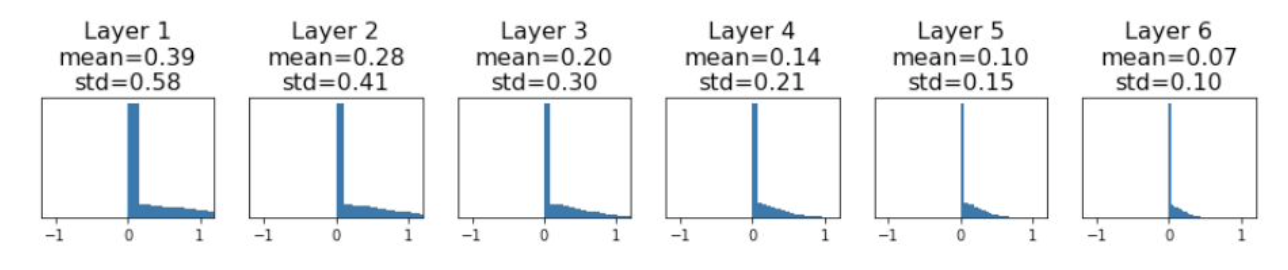
\includegraphics[width=.99\linewidth]{relu_init_x.png}
\end{center}
\end{frame}


\begin{frame}{А что с ReLU?}
\begin{columns}
	\begin{column}{.3\textwidth}	
		Инициализация Ксавье предполагает симметричную функцию активации
	\end{column}
	\begin{column}{.7\textwidth}
		dims = [{\color{green} 4096}] *  {\color{green} 7} \\
		hs = [ ] \\
		x = np.random.randn(  {\color{green} 16}, dims[  {\color{green} 0} ]) \\
		{\color{green} for} Din, Dout {\color{green} in zip}(dims[:  {\color{green} -1}], dims[ {\color{green} 1}:]): \\  
		\mbox{ } \hspace{5mm} W =  {\color{red} \textbf {np.sqrt(2/Din)} } * np.random.randn(Din, Dout) \\
		\mbox{ } \hspace{5mm} {\color{red} \textbf {x = np.max(0, x.dot(W))} } \\
		\mbox{ } \hspace{5mm} hs.append(x)
	\end{column}
\end{columns}
\begin{center}
	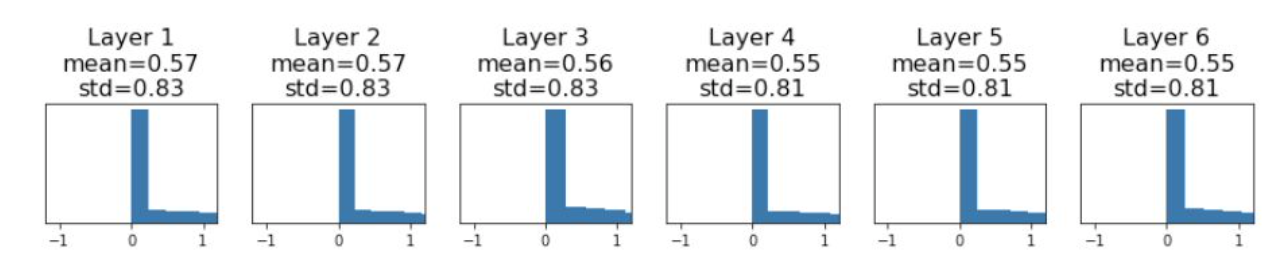
\includegraphics[width=.99\linewidth]{relu_init_xe.png}
\end{center}
\end{frame}



\begin{frame}{Инициализация Хе (2015)}
	\begin{multline*} 	
		\Var(h_i) = \Var(\sum_{i=1}^{n_{in}} w_i x_i) =  \sum_{i=1}^{n_{in}} \Var(w_i x_i) = \\ 
		= \sum_{i=1}^{n_{in}} [\E(x_i)]^2 \cdot \Var(w_i) + [\E(w_i)]^2 \cdot \Var(x_i)  + \Var(x_i) \cdot \Var(w_i)]  
		\only<2->{= \\  = \sum_{i=1}^{n_{in}} [\E(x_i)]^2 \cdot \Var(w_i) +  \Var(x_i) \cdot \Var(w_i)  =  \sum_{i=1}^{n_{in}} \Var(w_i) \cdot E(x_i^2)} 
		\only<3->{= \\  =  E(x^2)  \color{green} \cdot [n_{in} \cdot \Var(w)]}
	\end{multline*}

	\only<1-2>{	
	\begin{wideitemize}
		\item  Когда нет симметрии, можно занулить только второе слагаемое
	\end{wideitemize}}
\end{frame}


\begin{frame}{Инициализация Хе (2015)}
	\begin{align*} 	
		\Var(h_i)  & =   E(x_i^2)  \cdot [n_{in} \cdot \Var(w)] \\
	x_i & = \max(0; h_{i-1}) \\ 
	\end{align*} \pause 

	\only<2-> { Пусть $w_{i-1}$ распределены симметрично относительно нуля, тогда $h_{i-1}$ тоже будут симметрично распределены, тогда: }

	$$
	\only<3->{ E(x_i^2) = \frac{1}{2} \cdot \Var(h_{i-1}) }
	$$

	$$
	\only<4->{ \Var(h_i) =  \frac{1}{2} \cdot \Var(h_{i-1}) \cdot [n_{in} \cdot \Var(w)]  \Rightarrow \Var(w_i) = \frac{2}{n_{in}} }
	$$

	\vfill %
	\footnotesize
	{\color{blue} \url{https://arxiv.org/pdf/1502.01852.pdf}}
\end{frame}


\begin{frame}{TLDR: что на практике}
	\begin{wideitemize}
		\item  Для симметричных функций с нулевым средним используйте инициализацию Ксавье (Глорота) % {\color{green}  init="glorot\_uniform"} 
		\item  Для ReLU и им подобным инициализацию Хe %{\color{green} init="he\_uniform"} или {\color{green} init="he\_nomal"}
		\item  Эти две инициализации корректируют параметры распределений в зависимости от входа и выхода слоя так, чтобы поддерживать дисперсию равной единице
	\end{wideitemize}
\end{frame}


\begin{frame}{Тема инициализации сегодня активно исследуется}
\scriptsize{
	\begin{wideitemize} 
	\item Understanding the difficulty of training deep feedforward neural networks
	by Glorot and Bengio, 2010 
	
	\item Exact solutions to the nonlinear dynamics of learning in deep linear neural networks by Saxe et al, 2013 
	
	\item Random walk initialization for training very deep feedforward networks by Sussillo and Abbott, 2014 
	
	\item Delving deep into rectifiers: Surpassing human-level performance on ImageNet classification by He et al., 2015 
	
	\item Data-dependent Initializations of Convolutional Neural Networks by Krähenbühl et al., 2015 
	
	\item All you need is a good init, Mishkin and Matas, 2015 
	
	\item Fixup Initialization: Residual Learning Without Normalization, Zhang et al, 2019 
	
	\item The Lottery Ticket Hypothesis: Finding Sparse, Trainable Neural Networks, Frankle and Carbin, 2019
	\end{wideitemize}}
\end{frame}



\begin{transitionframe}
	\begin{center}
		\Huge  Попробуем новые трюки на практике? 
	\end{center}
%	\centering 
\includegraphics[scale = 0.25]{batcAlice.png}
\end{transitionframe}


\end{document}